\chapter{Guided Stable Dynamic Projections}
\blfootnote{This chapter is based on the paper ``Guided Stable Dynamic Projections'' \citep{Vernier2021}}
\label{ch:proj-algo}
% In Ch 5, we evaluated dyn projs from the dual perspective of visual quality and stability, just as we did for dyn TM algos in Chs 2-3. And, just as for the dyn TM algos, we found that there is no winning dyn projection that scores best for both vis quality and stability. In this chapter, similar to our earlier attempt in Ch 4 to improve dyn TMs, we aim to improve dyn projections from the perspective of the two aforementioned metrics.  For this, we propose two new dyn proj algos [….etc etc, link to the existing abstract]

\textit{
In Chapter \ref{ch:proj-eval}, we evaluated dynamic projections from the dual perspective of visual quality and stability, just as we did for dynamic treemap algorithms in Chapters \ref{ch:soft-eval}-\ref{ch:tree-eval}. And, just as for dynamic treemap algorithms, we found that there is no winning dynamic projection method that scores best for both visual quality and stability. In this chapter, similar to our earlier work in Chapter \ref{ch:git} to improve dynamic treemaps, we aim to improve dynamic projections from the perspective of the two aforementioned metrics. For this, we propose two new dynamic projection algorithms: PCD-tSNE and LD-tSNE. The former uses information given by the Principal Components of the data over all timesteps to stabilize tSNE. The latter makes use of landmarks that guide points through stable trajectories. We compare these two new algorithms with existing methods for dynamic projection, and show their advantages, following the benchmark proposed in Chapter \ref{ch:proj-eval}.
}

\vspace{5mm} %5mm vertical space


\noindent \textbf{Abstract:}
Projections aim to convey the relationships and similarity of high-dimensional data in a low-dimensional representation.
Most such techniques are designed for static data. When used for time-dependent data, they usually fail to create a stable and suitable low dimensional representation.
We propose two dynamic projection methods (PCD-tSNE and LD-tSNE) that use global guides to steer projection points. This avoids unstable movement that does not encode data dynamics while keeping t-SNE's neighborhood preservation ability. PCD-tSNE scores a good balance between stability, neighborhood preservation, and distance preservation, while LD-tSNE allows creating stable and customizable projections. We compare our methods to 11 other techniques using quality metrics and datasets provided by a recent benchmark for dynamic projections.
    
\section{Introduction}
%

Many domains produce datasets with large numbers of observations (also called samples or points) and attributes (also called measurements, dimensions, or variables). Dimensionality reduction techniques, also called projections, are an established tool for visualizing such datasets in a simplified, compact, and scalable way.

The literature on static projections -- that address the visualization of time-independent datasets -- is quite rich, with many techniques, surveys, and benchmarks on the subject\,\citep{Nonato2019,Espadoto19,sorzano14_survey,cunningham15_survey}. In contrast, far fewer techniques and comparisons thereof exist for projecting time-dependent datasets, in which the sample values change over time -- which is a much harder problem.

Besides faithfully capturing the data structure -- a desiderate shared with static projections -- dynamic projections also face the challenge of maintaining temporal coherence. Failing this will create false motion artifacts in the projection, which can mislead the user into thinking there are data changes where none exist, or conversely. Figure~\ref{fig:demo-instability} illustrates this: We have a 100-dimensional dataset of 2000 samples covering 10 distinct isotropic Gaussian distributions that collapse into 10 single points over 10 timesteps\,\citep{Rauber2016}. The images depict the results of three dynamic projection techniques (G-PCA, TF-PCA~\citep{pca}, and TF-tSNE\citep{vanderMaaten2008}) for this dataset, showing the trajectories of all data points over the ten timesteps. Knowing the dataset, we can tell that G-PCA renders quite faithfully the data dynamics and structure; TF-PCA creates an artificial amount of spiraling; and TF-tSNE creates a very large amount of apparently random and unstable motion that is not present in the data. If such variability in the projection results is seen for this simple, synthetic dataset, the choice of a good dynamic projection method for real-world datasets is clearly very hard.


% \red{There are different ways to project a dynamic dataset \red{(cite a few non-animation works)}, but we will focus on creating animation-like representations, where we project the $N$ samples of the original dataset into $2D$ space for each timestep $t$, as demonstrated in Fig.\,\ref{fig:animation}.}

% % https://docs.google.com/drawings/d/15hzYRNaO8qreoUQrndlu_6f5Sn1c8ebI0HuE5yEEOVY/edit
% \begin{figure}[!h]\centering
%   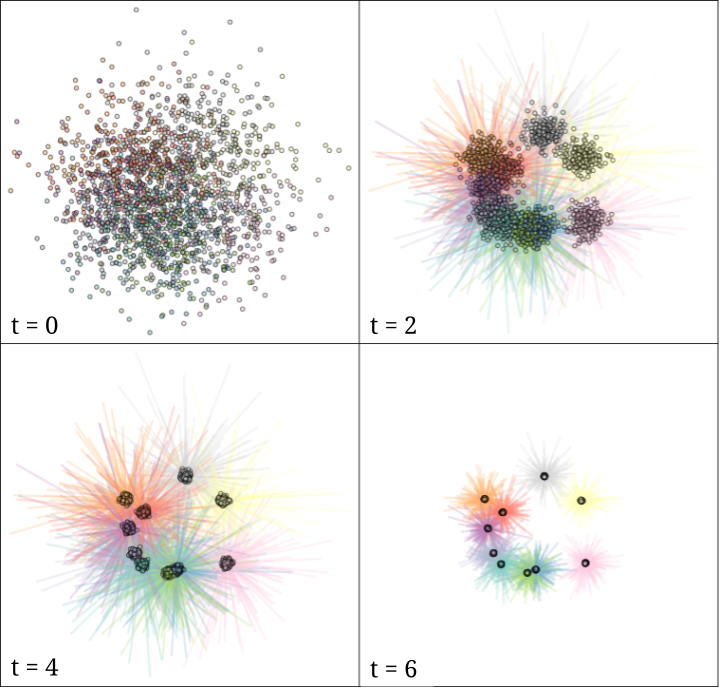
\includegraphics[width=\linewidth]{figures/projection-algorithm/gaussians-pca-s4.png}
%   \caption{caption}
%   \label{fig:animation}
% \end{figure}

% https://docs.google.com/drawings/d/1XENnHkpmsl6AqJfx5l2b-H4bSuKonbjgjYY_E599Q5c/edit
\begin{figure*}[h]
 \centering
 \includegraphics[width=\linewidth]{figures/projection-algorithm/demo-instability-trails-rebuttal-with-color-3.eps}
%  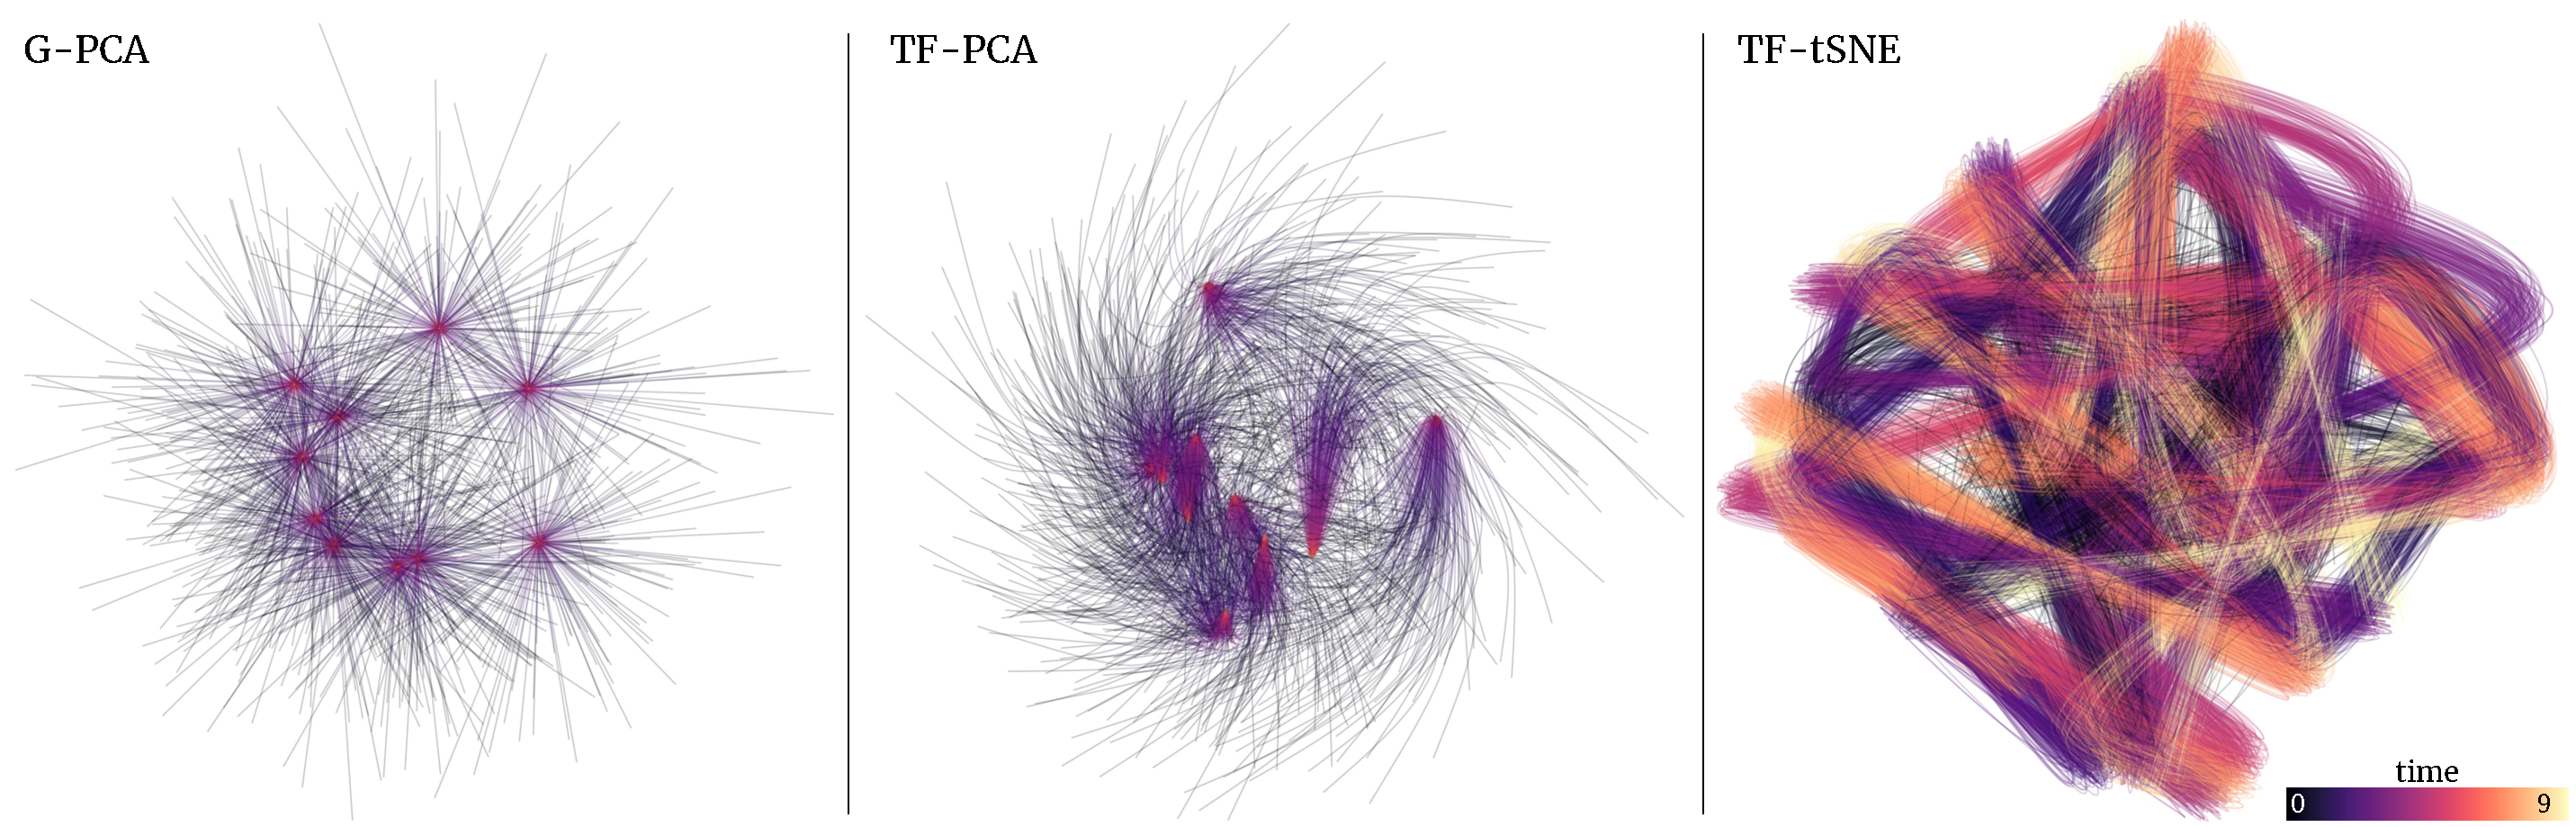
\includegraphics[width=0.48\linewidth]{figures/projection-algorithm/demo-instability-trails-rebuttal-with-color.pdf}
 \caption{A time-dependent collapsing 100-dimensional 10-Gaussian-distributions dataset (2000 points) is visualized by three projection methods. Point trails are colored by time (top) and class (bottom). The images show increasing amounts of instability artefacts.}
 \label{fig:demo-instability}
 \vspace{-0.15cm}
\end{figure*}

Motivated by these challenges of understanding and quantifying the quality of dynamic projections, \cite{Vernier2020} evaluated nine such techniques, and came to the conclusion that there is no perfect method, and that an inherent trade-off between stability and spatial quality (i.e., neighborhood and distance preservation) exists. The methods that scored the best on both criteria were autoencoder-based methods and Global PCA. Neighborhood-based methods, such as t-SNE and UMAP, strongly showed a lack of stability. At the same time, these are among the favorite methods for static projection, given their high capability in preserving data structure.

We aim to cover the above-identified gap by proposing ways to add stability to the neighborhood preservation ability of static projections, in particular t-SNE. We propose two approaches that use global influences to steer projected points:
Our first method, LD-tSNE, offers similar flexibility in steering dynamic projections via landmarks as known for static projections, and also reaches good quality values. Our second method, PCD-tSNE, increases neighborhood influences atop an already stable Global PCA dynamic projection, scoring better than all compared counterparts in terms of spatial quality combined with stability. The global influence of both methods can be controlled via simple user parameters to find the best balance between stability and spatial quality. We compare our methods with 11 existing dynamic projections on a benchmark of 10 high-dimensional datasets using 12 metrics for both spatial quality and stability. 

Section~\ref{sec:background} overviews related work on dynamic projections of high-dimensional data. Section~\ref{sec:methods} introduces our two new methods. Section~\ref{sec:experimental-setup} presents the experimental setup we used in comparing our new methods with existing ones. Section~\ref{sec:results} presents and discusses the evaluation results. Finally, Section~\ref{sec:conclusion-5} concludes the paper.

  
%-------------------------------------------------------------------------
\vspace{-0.15cm}
\section{Related work}
\label{sec:background}

\subsection{Preliminaries}
%
We first introduce some notations. Let
$\mathbf{x} \in \mathbb{R}^n$
be an $n$-dimensional sample (also called data point or observation). A timestep $\mathbf{D}^t = \{\mathbf{x}_i^t\}$ of our data consists of a set of $N$ samples $\mathbf{x}_i^t$, $1 \leq i \leq N$, 
measured at the same time moment $t$. A dynamic dataset $\mathbf{D}$ is a list of $T$ timesteps $\mathbf{D}= ( \mathbf{D}^{t} ), 1 \leq t \leq T$. For simplicity of exposition and implementation, but without loss of generality, we consider next that the sample count $N$ is constant over time. In this case, $\mathbf{D}$ can be represented as a set of $T$ $N$-by-$n$ matrices, one per timestep $t$.

A projection technique is a function $P: \mathbb{R}^{n} \rightarrow \mathbb{R}^{q}$, where $q \ll n$. For visualization purposes, $q \in \{2,3\}$. Since 2D projections are by far the most commonly used, we next only consider the case $q=2$. We denote the projection of sample $\mathbf{x}$ by $P(\mathbf{x})$. For a timestep $t$, let $P(\mathbf{D}^{t}) = \{ P(\mathbf{x}^t) | \mathbf{x}^t \in \mathbf{D}^{t} \}$ be the 2D scatterplot of the projections of all points in
$\mathbf{D}^{t}$. Finally, let $P(\mathbf{D})$ be the set of $T$ scatterplots for all timesteps of dataset $\mathbf{D}$. These can be rendered as animations (see additional material\,\citep{repo-guided}), trail sets (as in Fig. \ref{fig:demo-instability}), small multiples\,\citep{Rauber2016}, or other visual encodings. 


\subsection{Visualization of high-dimensional data}
\label{sec:rw_vis_dynamic}
%

Visualization of static high dimensional data\,\citep{Liu2017} is a well studied topic populated with many techniques such as parallel coordinate plots\,\citep{Inselberg1990}, table lenses\,\citep{Rao2003}, scatterplot matrices\,\citep{Becker1996}, and dimensionality reduction (DR) methods or projections\,\citep{vanderMaaten2009}. Compared to other methods, projections scale visually very well, being able to accommodate datasets of millions of samples and hundreds up to thousands of dimensions in limited screen space. Several quality metrics have been proposed to gauge how faithfully projections capture the structure of high-dimensional data, \emph{e.g.}, trustworthiness and continuity\,\citep{venna06}, normalized stress and Shepard diagrams\,\citep{Joia2011}, neighborhood hit\,\citep{Paulovich2008}, class consistency\,\citep{tatu10}, and distance consistency\,\citep{sips09}. Tens of different projection algorithms exist for static data; detailed taxonomies of such methods, benchmarks, and qualitative and quantitative evaluations are available in a range of surveys\,\citep{Nonato2019,Espadoto19,fodor02_survey,cunningham15_survey,sorzano14_survey,vanderMaaten2009}.

%Comparatively few works use projections to explore temporal (time-dependent) high-dimensional data. Most importantly, few authors explicitly propose techniques and strategies for creating stable projections for temporal\,\citep{Rauber2016,Vernier2020} and for streaming data\,\citep{Neves2020}.

\subsection{Strategies for dynamic projections} 
\label{sec:taxonomy}
%
All current dynamic projection techniques that we are aware of are based on methods that were initially designed for static data. These base methods are adapted to achieve two goals: (a) obtaining good \emph{spatial quality}, measured by the various static projection metrics outlined earlier in Sec.~\ref{sec:rw_vis_dynamic}; and (b) obtaining good \emph{stability}, defined as the ratio between changes, over time, of the projection $P(\mathbf{D})$ \emph{vs} changes of the data $\mathbf{D}$\,\citep{Vernier2020}. Besides projections, similar definitions of stability have been used to quantify dynamic treemapping algorithms\,\citep{vernier_treemap,vernier18software}.  We next propose to classify these techniques as a function of how they `adapt' the underlying base (static) projection algorithm, denoted further $P_B$, to handle spatial quality and stability for dynamic data.\\

%A number of these strategies were proposed by Rauber \emph{et al.} \citep{Rauber2016} using t-SNE as testbed, but were not implemented or quantitatively tested. 
%Later, Vernier \emph{et al.} \citep{Vernier2020} explored the idea further, benchmarking the proposed methods and applying these strategies to other base algorithms. These strategies, according to our taxonomy, are:

\noindent\textbf{Per-timeframe (TF):} 
In this simplest strategy, $P_B$ is applied to each timestep $\mathbf{D}^t$ to create an independent projection $P_B(\mathbf{D}^t)$. Hence, $P(\mathbf{D}) = ( P_B(\mathbf{D}^t))_{ 1 \leq t \leq T}$. In other words, the base method $P_B$ is not allowed to ``look at the past or future'' when projecting a given timestep $t$ -- it only sees the data in $\mathbf{D}^t$. Given the popularity of PCA\,\citep{pca}, t-SNE\,\citep{vanderMaaten2008}, and UMAP\,\citep{umap}, the per-timeframe strategy is often used for these base projections, leading to variants we call next TF-PCA, TF-tSNE, and TF-UMAP, respectively. Several further variations of this strategy exist. \cite{bsk16} propose time curves which connect consecutive positions $P_B(\mathbf{x}_i^t)$ of the same point $i$ for all moments $t$, using MDS for $P_B$. Similar curves have been used by \cite{bws12} (using PCA for $P_B$). \cite{Brich2020} use time curves and argue for the pro's and con's of PCA \emph{vs} MDS for $P_B$. However, none of the studied base projections was found ideal concerning stability and spatial quality. At a more general level, the same strategy was used to connect different 2D scatterplots created by other means than projections\,\citep{hkf16}. \cite{Jackle2016} use MDS for $P_B$ to project all $n$ spatial dimensions of $\mathbf{D}$ to a single dimension and use the second dimension of the screen space to map time. 
Overall, the per-timeframe strategy favors spatial quality, which can be as high as delivered by $P_B$. However, stability can be (very) low since $P_B$ is applied independently to the timeframes. \\

\noindent\textbf{Global (G):}
At the other end of the spectrum, global methods apply $P_B$ to the entire dataset, and then separate the projected points based on their timesteps, \emph{i.e.}, $P(\mathbf{D}) = (\{\mathbf{y}^t \in P_B(\mathbf{D})\})_{1 \leq t \leq T}$, where $\mathbf{y}^t = P_B(\mathbf{x}^t)$ and $\mathbf{x}^t \in \mathbf{D}^t$. Like per-timeframe, this strategy is also simple to implement. It maximizes stability by construction. As such, many applications use this strategy, \emph{e.g.} \cite{Hu2010} that project 72-dimensional human body keypoints using LLE, or \cite{Fujiwara2018} who project entire dimensions (time series) using MDS and t-SNE for computer performance analysis. The latter method was also extended to use PCA and UMAP as $P_B$\,\citep{Fujiwara2020}.

When $\mathbf{D}$ is large, either in terms of number of samples or number of timesteps, computing a single projection $P_B(\mathbf{D})$ can be expensive. Also, the spatial quality of global techniques is typically lower than for the per-timeframe strategy since $P_B$ now has to optimize the relative placement of points in \emph{all} timeframes, even if such points never co-exist at the same time. Out-of-sample projection (OOS) methods can help with these issues. Simply put, an OOS technique $P$ is constructed to optimize the projection of a subset $\mathbf{D}_s \subset \mathbf{D}$ according to one's desired quality metrics. Next, $P$ is used to extrapolate the projection to the entire $\mathbf{D}$. Out-of-sample strategies have been proposed for many static projection methods\,\citep{oos}. Recently, \cite{MateusEspadoto} have shown how to use deep learning to construct out-of-sample approximations of any static projection technique. Hence, OOS techniques can be used to accelerate and potentially increase the quality of global projection methods. However, the challenge is in how to select the small subset $\mathbf{D}_s$ so as to represent well the entire time-dependent dataset $\mathbf{D}$. To our knowledge, no studies of this aspect exist for dynamic projections.\\

\noindent\textbf{Continuous (C):} This strategy applies to base methods that iteratively optimize neighborhood configurations, such as t-SNE and UMAP. In the following, we call these variants C-tSNE and C-UMAP, respectively. The projection $P(\mathbf{D}^{t})$ continues the gradient descent from the positions of the previous timestep $P(\mathbf{D}^{t-1})$, with the updated cost function for $t$. This reduces significantly the non-deterministic behavior created by removing consecutive initialization steps. Still, this can fail to produce stable projections as points are still allowed to move significantly during optimization. Dynamic t-SNE (D-tSNE)\,\citep{Rauber2016} aims to alleviate this by adding a penalty term to the continuous strategy using t-SNE for $P_B$. This limits, up to a certain extent, too large point movements between consecutive timesteps.
Incremental PCA\,\citep{ross08} projects points in a streaming fashion and is therefore amenable to project time-dependent data. \cite{Fujiwara2020} further increase incremental PCA's stability by using Procrustes analysis to align consecutive projections, a method also proposed independently by \cite{Joia2011}. \cite{Neves2020} propose Xtreaming, an incremental technique that handles streaming high-dimensional data by continuously adapting UPDis\,\citep{updis}, a projection with out-of-sample capability, thus, good stability. Overall, continuous strategies achieve a good balance between spatial quality and stability. However, this balance can be hard to tune in practice. 

Vernier \emph{et al.}'s evaluation\,\citep{Vernier2020} found that PCA and (Variational) Autoencoders with the global strategy -- called next G-PCA, G-VAE, and G-AE respectively -- were the best-suited methods for projecting temporal data. The global strategy, however, does not seem to work well with graph or neighborhood-based methods, such as t-SNE and UMAP -- we denote these methods next as G-tSNE and G-UMAP, respectively. 

%-------------------------------------------------------------------------
\section{Guided methods for dynamic projection}
\label{sec:methods}
%
Many guided methods exist in the static projection literature\,\citep{Nonato2019,sorzano14_survey}. Simply put, all these methods select a subset of samples $\mathbf{L} \subset \mathbf{D}$ to create $P$, by extrapolating $P(\mathbf{L})$ to $P(\mathbf{D})$. Conceptually speaking, the continuous strategy (Sec.~\ref{sec:taxonomy}) can be seen as a type of guidance, where $P(\mathbf{D}^{t+1})$ is steered by the earlier projection $P(\mathbf{D}^{t})$. Similarly, the out-of-sample global strategy (Sec.~\ref{sec:taxonomy}) can be seen as a type of guidance where $P(\mathbf{D}_s)$ steers $P(\mathbf{D})$. However, even though this works for simple datasets, when the data present complex dynamics and large changes over time, existing continuous strategies become too restrictive. We propose two new guided methods for dynamic projection that use global influences (landmarks or suggested placements) to steer and stabilize the projection while still accounting for neighborhood preservation. The two methods use t-SNE as base projection given (a) t-SNE's high popularity for the static projection case; and (b) the difficulty of using t-SNE in a dynamic context (see Sec.~\ref{sec:taxonomy}), which we want to overcome.
Importantly, while guided strategies mainly aim to address \emph{scalability} for static projections, our different aim of using guidance is to address \emph{spatial quality} and \emph{stability}. 

%-------------------------------------------------------------------------
\subsection{Landmark Dynamic t-SNE (LD-tSNE)}
\label{sec:ld-tsne}
%
One idea that has been successfully used in the static case, and can be utilized to our advantage for dynamic data, is the use of \emph{landmarks}. 
Landmarks or similar control point-based mechanisms are well known and have been used to aid different tasks on static data. Examples include performance improvement\citep{Pekalska1999,DeSilva2003,DeSilva2004,Vladymyrov2013,Paulovich2008,Kruiger2017a}, support of out-of-sample capability\citep{Boytsov2017,Policar2019}, and projection customization\citep{Joia2011,updis}.
Yet, we are not aware of any work that combines landmarks or control points to stabilize \emph{dynamic} projections. We use landmarks to give the base projection $P_B$ method a sense of global structure, in an attempt to reduce the instability inherent to neighborhood-based projection techniques such as t-SNE.

Two main aspects must be considered when using landmarks as guides: how to generate the landmarks and how to use the landmarks to steer points, as follows.\\

\vspace{-0.15cm}
\noindent\textbf{Landmark generation:} Each landmark $\mathbf{l}=\left(\mathbf{l}^n, \mathbf{l}^q\right)$ consists of a high-dimensional component $\mathbf{l}^n \in \mathbb{R}^n$ and a component $\mathbf{l}^q \in \mathbb{R}^q$ in the projection space.
It is important that the set $\mathbf{L} = \{ l^n \}$ captures well the structure of the high-dimensional dataset $\mathbf{D}$, otherwise the ``steering'' may become uneven. There are different ways of achieving this goal\,\citep{DeSilva2005}. For simplicity and speed, we opted to create $\mathbf{L}$ by randomly sampling $k$ points from $\mathbf{D}$, where $k$ is a fraction of the size of $\mathbf{D}$. For most of our tests, we set $k=N$, \emph{i.e.}, the number of points in a timeframe (see Appendix in supplementary material). To generate the low-dimensional points $\mathbf{l}^q$, we simply project $\mathbf{L}$ using a user-chosen method. We experimented here with both PCA and t-SNE, and selected the landmark projection which yielded the best results (see Appendix in supplementary material).\\

\vspace{-0.15cm}
\noindent\textbf{Landmark steering:} The first step towards steering is to select a neighborhood-based projection technique to use. We chose here t-SNE due to its popularity and previous good results in extending it for dynamic data\,\citep{Rauber2016}. To describe how steering takes place, let us consider the original t-SNE cost function, given by the Kullback-Leibler (KL) divergence between the joint-probability distributions $\mathcal P$ and $\mathcal Q$ that describe point-neighborhoods in $\mathbb{R}^n$, respectively $\mathbb{R}^q$
%
\begin{equation}
C_{tsne} = D_{KL}\left(\mathcal{P}||\mathcal{Q}\right) =  \sum_{i=1}^{N} \sum_{j\neq i} p_{i j} \log \frac{p_{i j}}{q_{i j}},
\label{eqn:c_tsne}
\end{equation}
%
where $ p_{ij}=\frac{p_{i | j}+p_{j | i}}{2 N}$ models the distance of two points $\mathbf{x}_i$ and $\mathbf{x}_j$ in $\mathbb{R}^n$ and
%
$$ p_{j | i}=\frac{\exp \left(-\left\|\mathbf{x}_{i}-\mathbf{x}_{j}\right\|^{2} / \left(2 \sigma_{i}^{2}\right)\right)}  
{\sum_{k \neq i}^{N} \exp \left(-\left\|\mathbf{x}_{i}-\mathbf{x}_{k}\right\|^{2} /\left(2 \sigma_{i}^{2}\right)\right)}. $$
%
Here, $p_{j|i}$ can be seen as a relative measure of similarity based on the local neighborhood of a point $\mathbf{x}_i$. The effective number of neighbors considered for each point is given indirectly by a user-chosen perplexity value $\mu$: The value of $\sigma_i$ is computed so that, for the user-given $\mu$ and each $i$, $\mu=2^{-\sum_{j}^{N} p_{j | i} \log _{2} p_{j | i}}$.

A Student's t-distribution with one degree of freedom is used to compute the joint-probability distribution in $\mathbb{R}^q$ as
%
$$q_{i j}=\frac{\left(1+\left\|\mathbf{y}_{i}-\mathbf{y}_{j}\right\|^{2}\right)^{-1}}{\sum_{k, i \neq k}\left(1+\left\|\mathbf{y}_{i}-\mathbf{y}_{k}\right\|^{2}\right)^{-1}}.
$$
The gradient of the cost function, given by
%
\begin{equation}
 \frac{\partial C_{tsne}}{\partial \mathbf{y}_{i}}=4 \sum_{j}\left(p_{i j}-q_{i j}\right)\left(\mathbf{y}_{i}-\mathbf{y}_{j}\right)\left(1+\left\|\mathbf{y}_{i}-\mathbf{y}_{j}\right\|^{2}\right)^{-1} 
 \label{eqn:grad_tsne}
\end{equation}
%
is used to incrementally move the points $\mathbf{y}_i$ to reduce the cost $C_{tsne}$.

To add landmark influence to t-SNE we will, similarly to \cite{Rauber2016}, add a second term to the cost function. In their work, the extra term was used to penalize \emph{any} kind of 2D movement. In our case, we want to \emph{guide} the placement of points $\mathbf{y}_i$ based on the similarity of $\mathbf{x}_i$ with the landmarks $\mathbf{l}^n$. Figure~\ref{fig:ldtsne} illustrates these global and local influences. In Fig.~\ref{fig:ldtsne}a, the landmarks in $\mathbf{L}$ (light blue) produce attraction and repulsion forces to guide the placement of the red point $\mathbf{y}_i$. In Fig.~\ref{fig:ldtsne}b, the remaining points $\mathbf{y}_j$, $j \neq i$ (gray in the figure), exert similar forces, influencing and being influenced by $\mathbf{y}_i$, just like in a regular t-SNE projection.

We weigh the global and local influences by a factor $\lambda  \in [0, 1]$ giving the total cost function
%
\begin{equation}
C = (1-\lambda)C_{tsne} + \lambda C_{landmarks}. 
\label{eqn:c_ours}
\end{equation}
%
In the above, $C_{landmarks}$ is similar to the original t-SNE cost function $C_{tsne}$. However, instead of considering $p_{ij}$ for all pairs of points in $\mathbf{D}$ or $\mathbf{D}^t$, we let only the landmarks $ \mathbf{l} \in L$ act upon each $\mathbf{y}_i$, \emph{i.e.} 
%
\begin{equation}
C_{landmarks}=\sum_{i} \sum_{l \in L} p_{i|l} \log \frac{p_{i|l}}{q_{il}}.
\label{eqn:c_land}
\end{equation}
%
For these influences to work consistently through all time steps $t$, several aspects differ from the original t-SNE. In Eqn.~\ref{eqn:c_land}, we use the \emph{asymmetric} $p_{i|l}$ instead of the symmetric $p_{il}$ used in Eqn.~\ref{eqn:c_tsne}. Indeed, we want the landmarks to influence the points, not the other way round. Secondly, for the computation of $\sigma_l$ for each landmark, we only take into consideration the landmark points $\mathbf{L}$. These two modifications ensure that the forces are consistent and do not fluctuate depending on the local density of points in $\mathbf{D}$ or $\mathbf{D}^t$.

From Eqns.~\ref{eqn:grad_tsne}, \ref{eqn:c_ours}, and~\ref{eqn:c_land}, we find the gradient of $C$ as
%
\begin{equation*}
  \begin{aligned}
    \frac{\partial C}{\partial \mathbf{y}_{i}} =(1-\lambda)\left(4 \sum_{j}\left(p_{i j}-q_{i j}\right)\left(\mathbf{y}_{i}-\mathbf{y}_{j}\right)\left(1+\left\|\mathbf{y}_{i}-\mathbf{y}_{j}\right\|^{2}\right)^{-1}\right) \\
    +\lambda\left(4 \sum_{l \in L}\left(p_{i | l}-q_{i j}\right)\left(\mathbf{y}_{i}-\mathbf{y}_{j}\right)\left(1+\left\|\mathbf{y}_{i}-\mathbf{y}_{j}\right\|^{2}\right)^{-1}\right).
  \end{aligned}
\end{equation*}


To accelerate convergence, improve initialization, and create tighter clusters, exaggeration terms are used \citep{vanderMaaten2008,vanderMaaten2015,Linderman2017,Linderman2017a}. These are scalars that multiply $p_{i j}$, suggesting greater similarity between points than $\mathcal P$ captures. We do the same by adding two factors $\alpha$ and $\beta$ to grant additional influence on how much points in $\mathbf{D}^t$ affect each other ($\alpha = $ local), respectively how much the landmarks ``pull'' the projected points ($\beta$ = global), leading to the final cost gradient
%
\begin{equation*}
 \begin{aligned}
  \frac{\partial C}{\partial \mathbf{y}_{i}} =(1-\lambda)\left(4 \sum_{j}\left(\alpha p_{i j}-q_{i j}\right)\left(\mathbf{y}_{i}-\mathbf{y}_{j}\right)\left(1+\left\|\mathbf{y}_{i}-\mathbf{y}_{j}\right\|^{2}\right)^{-1}\right) \\
  +\lambda\left(4 \sum_{l \in L}\left(\beta p_{i | l}-q_{i j}\right)\left(\mathbf{y}_{i}-\mathbf{y}_{j}\right)\left(1+\left\|\mathbf{y}_{i}-\mathbf{y}_{j}\right\|^{2}\right)^{-1}\right).
 \end{aligned}
\end{equation*}
%

%
% drawing at https://docs.google.com/drawings/d/1eweekZraQIyAtnmhA89MoFp0af11ic91d_qjd08Je5M/edit
\begin{figure}[h]\centering
  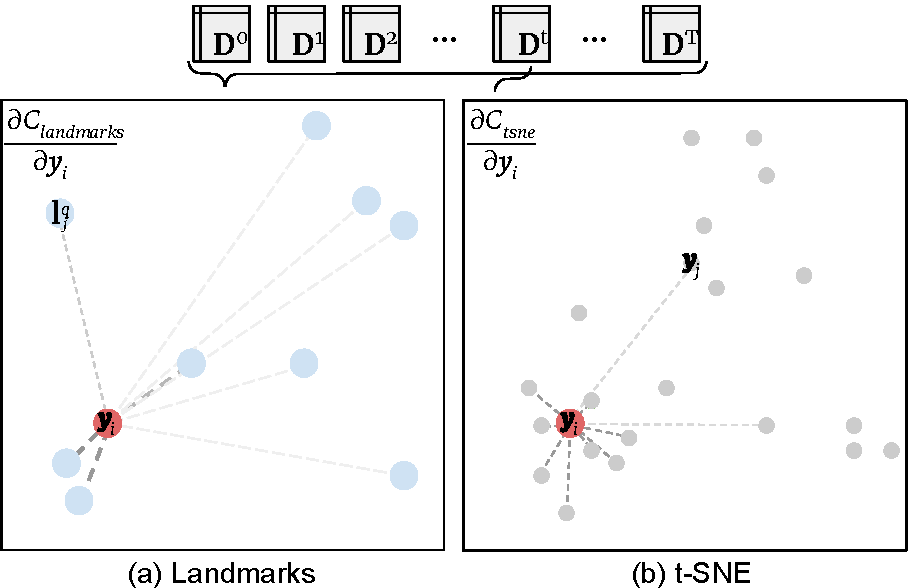
\includegraphics[width=\linewidth]{figures/projection-algorithm/ldtsne.pdf}
  \caption{Effect of landmarks (a) and regular projection points (b) upon a point $\mathbf{y}_i$ in LD-tSNE. See Sec.~\ref{sec:ld-tsne}.}
  \label{fig:ldtsne}
\end{figure}

Regarding algorithmic complexity, the original unoptimized implementation of the t-SNE method is $\mathcal{O}(n^2)$ for both computation and memory\,\citep{vanderMaaten2008}. Our LD-tSNE algorithm has an additional cost $\mathcal{O}(ln)$ given by the interaction of the landmarks with the points in the projection, where $l$ is the number of landmarks and $n$ the number of points in the projection. Therefore, the final time and memory complexity are given as $\mathcal{O}(n^2 + ln)$, or, since $n^2$ dominates the cost, LD-tSNE can be considered $\mathcal{O}(n^2)$. 

%-------------------------------------------------------------------------
\subsection{Principal Component Dynamic t-SNE (PCD-tSNE)} 
\label{sec:pcd-tsne}
%
Our second dynamic projection, PCD-tSNE, is a guided method that allies the stability of G-PCA with the neighborhood preservation capabilities of t-SNE.
Just like D-tSNE and LD-tSNE, it includes an additional term to the t-SNE cost function that adds stabilization to the otherwise unstable C-tSNE. 

The first step in PCD-tSNE is to compute a projection matrix $W$ constructed from the top-$q$ eigenvectors of the covariance matrix of $\mathbf{D}$. Simply put, $W$ describes the (two, in our case) orthogonal axes of largest data variation over the whole dataset. For each point $\mathbf{x}_i \in \mathbf{D}$, we apply a transformation $\mathbf{x}_i W$ to map $\mathbf{x}_i$ to $\mathbb{R}^q$. More specifically, this places $\mathbf{x}_i$ exactly as G-PCA would, which was proven earlier\,\citep{Vernier2020} to create \emph{stable} projections.

The placement of each projection point $\mathbf{y}_i$ is next given by two factors (see Fig.~\ref{fig:pcdtsne}): an attraction to the position $\mathbf{x}_i W$, marked in light blue in Fig.~\ref{fig:pcdtsne}a; and the influence of all other points in $\mathbf{D}^t$ 
upon $\mathbf{y}_i$, as given by tSNE, these points being shown in gray in Fig.~\ref{fig:pcdtsne}b. With these elements, the gradient of our cost function is given by:  

% It uses the pricipal components of $\mathbf{D}$ to guide the placement of points by trying to minimize the distance of a point $y_i$ to the point $x_i W$ (i.e., G-PCA position of $x_i$ given $\mathbf{D}$), where $W$ is the projection matrix constructed from the top-$q$ eigenvectors of $\mathbf{D}$.
% The gradient is therefore given by:
%

\begin{equation}
\label{eqn:pcd-tsne}
\frac{\partial C}{\partial \mathbf{y}_{i}} = (1-\lambda) \frac{\partial C_{tsne}}{\partial \mathbf{y}_{i}} + \lambda \|\mathbf{y}_i - \mathbf{x}_i W \|.
\end{equation}

%
Here, $\lambda \in [0,1]$, similarly to LD-tSNE, weighs the balance of local and global influences. More specifically, by adjusting $\lambda$, we can achieve an exact C-tSNE projection ($\lambda=0$), an exact G-PCA projection ($\lambda=1$), or a projection in between these variants.

%% \red{pc scaling}

% drawing at https://docs.google.com/drawings/d/1mXEM_zlZUVlTNV5UF2N3M5ZlHzy08v1lBFvJipaSt90/edit
\begin{figure}[h]\centering
  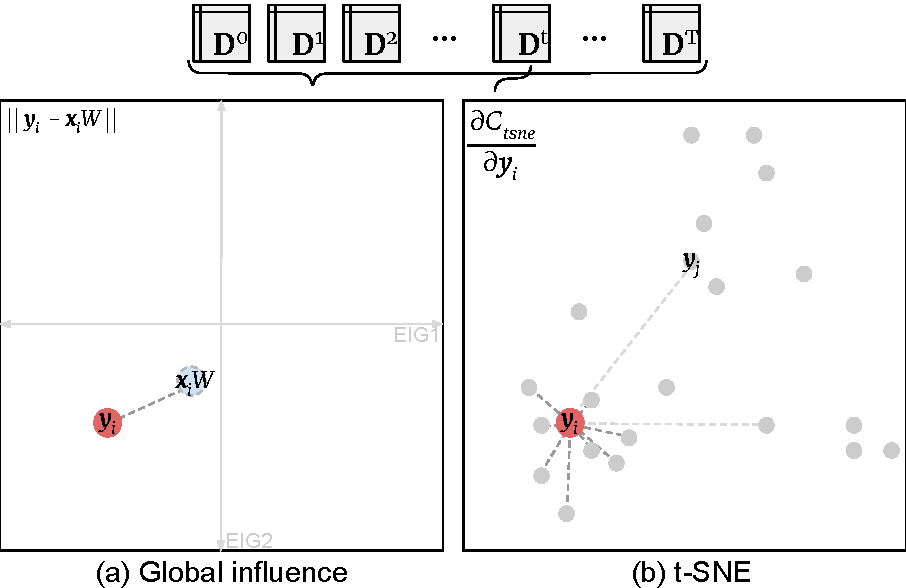
\includegraphics[width=\linewidth]{figures/projection-algorithm/pcdtsne.pdf}
  \caption{Effect of global influence (a) and regular projection points (b) upon a point $\mathbf{y}_i$ in PCD-tSNE. See Sec.~\ref{sec:pcd-tsne}.}
  \label{fig:pcdtsne}
\end{figure}

Regarding complexity, for PCD-tSNE, the first step is to compute the top-2 eigenvectors of the original data. There are many numerical methods designed to efficiently perform this computation  with cost as low as $\mathcal{O}(kn)$ for $k$ singular values \citep{svd-complexity,cline2006computatio}.
Once the PCD-tSNE optimization starts, the additional term introduced on Equation \ref{eqn:pcd-tsne} represents a simple convex function, which means that convergence is reached efficiently and PCD-tSNE performs similarly to C-tSNE, that is, in $\mathcal{O}(n^2)$ time.


%-------------------------------------------------------------------------
\section{Evaluation procedure} 
\label{sec:experimental-setup}
%
We next present our evaluation of the two proposed dynamic projection methods, LD-tSNE and PCD-tSNE. For the evaluation, we started with the benchmark in \cite{Vernier2020}, which is to our knowledge the only benchmark dedicated specifically to dynamic projections. The implementation of per-timeframe and global methods were provided by\,\cite{Vernier2020}; D-tSNE was provided by\,\cite{Rauber2016};  the remaining techniques considered in our evaluation (Sec.~\ref{sec:methods}) were implemented by ourselves. All source code, datasets, and obtained results can be found in our online repository\,\citep{repo-guided}. 

\subsection{Methods}
\label{sec:eval-methods}

The \cite{Vernier2020} benchmark (described in the previous chapter) contained 9 methods -- five global ones (G-AE, G-VAE, G-tSNE, G-UMAP, G-PCA), three per-timeframe ones (TF-tSNE, TF-UMAP, TF-PCA), and one continuous (D-tSNE).  Atop of those we added C-tSNE and C-UMAP, and the two newly proposed methods, LD-tSNE and PCD-tSNE. The parameters used in the benchmark are available in the supplemental material.

\subsection{Quality Metrics}
\label{sec:metrics}
%
Following \cite{Vernier2020} and\,\cite{Espadoto19}, we used 8 \emph{spatial} and 4 \emph{temporal} quality metrics, as follows. Temporal metrics measure the correspondence of movement of projection points in $\mathbb{R}^q$ with regard to their change in the data space $\mathbb{R}^n$ space, \emph{i.e.}, stability. 

\subsubsection{Spatial metrics}
\label{sec:spatial}

Spatial metrics measure how well a projection maps the underlying high-dimensional data, and can be divided into neighborhood preservation metrics ($S_{NP}, S_{NH}, S_{Trust}, S_{Cont}$) and distance preservation metrics ($S_{Stress}, S_{Pearson}, S_{Spearman}, S_{Kendall}$ ). Note that these do not necessarily relate to how humans perceive the projection \citep{Wang2018}.\\

\noindent\textbf{Neighborhood preservation ($S_{NP}$)} is the fraction of the $k$-nearest neighbors of $\mathbf{x} \in \mathbf{D}$ whose projections are in the $k$-nearest neighbors of $P(\mathbf{x})$.\\

\noindent\textbf{Trustworthiness ($S_{Trust}$)} measures how well the $k$ nearest neighbors $\nu^k(P(\mathbf{x}))$ of a projected point $P(\mathbf{x})$ match the $k$ nearest neighbors $\nu^k(\mathbf{x})$ of a data point $\mathbf{x}$, specifically, how \emph{few} missing neighbors\,\citep{Martins2014} a projected point has. If $U^k(\mathbf{x})$ is the set of points in $\mathbf{D}$ that project in $\nu^k(P(\mathbf{x}))$ but are not in $\nu^k(\mathbf{x})$,
and $r^P(\mathbf{x},\mathbf{y})$ is the rank of $\mathbf{y}$ in the ordered set of nearest neighbors $\nu^k(P(\mathbf{x}))$, trustworthiness is defined as \linebreak
$1-\frac{2}{N k(2 N-3 k-1)} \sum_{x=1}^{N} \sum_{y \in U^k(\mathbf{x})}(r^P(\mathbf{x}, \mathbf{y})-k)$.\\
%$1 - \sum_{\mathbf{y} \in U^k(\mathbf{x})}(r(\mathbf{x}, \mathbf{y})-k)$.

\noindent\textbf{Continuity ($S_{Cont}$)} measures how \emph{many} missing neighbors a projected point has. Let $V^k(\mathbf{x})$
be the points that are in $\nu^k(\mathbf{x})$ but do not project in $\nu^k(P(\mathbf{x}))$. Let ${r}(\mathbf{x}, \mathbf{y})$ be the rank of $\mathbf{y}$ in the ordered set of neighbors $\nu^k(\mathbf{x})$. Continuity is then defined as \linebreak
$1-\frac{2}{N k(2 N-3 k-1)} \sum_{x=1}^{N} \sum_{y \in V^k(\mathbf{x})}({r}(\mathbf{x}, \mathbf{y})-k)$.\\
%$1- \sum_{\mathbf{y} \in V^k(\mathbf{x})}({r}(\mathbf{x}, \mathbf{y})-k)$.
% We compute all the above metrics locally for each projection point $P(\mathbf{x})$ and, for presentation purposes, average them next as required by the analysis at hand.

\noindent\textbf{Neighborhood hit ($S_{NH}$)} is the fraction of the $k$-nearest neighbors of a projected point $P(\mathbf{x})$ that have the same class label as $P(\mathbf{x})$. Since we use labeled datasets with reasonably well-separated classes in $\mathbb{R}^n$ (see next Sec.~\ref{sec:datasets}), a projection $P$ that is good for class-separation tasks should have a high $S_{NH}$ value.\\

All the above metrics range in $[0,1]$, with 1 indicating optimal value. 
We compute $S_{NP}$, $S_{Trust}$, and $S_{Cont}$ for multiple (20) neighborhood sizes equally spread between $k=1\%$ and $k=20\%$ of the point count $N$. For $S_{NH}$, we use 20 values for $k$, ranging from 0.25\% to 5\% of $N$. 
We next average the results for different neighborhood sizes $k$, following\,\citep{Vernier2020,Martins2015}.\\


\noindent\textbf{Normalized stress ($S_{Stress}$)} measures the pairwise difference of distances of points in $\mathbf{D}$ and $P(\mathbf{D})$. We define $S_{Stress}$ as $\sum_t \sum_{ij}(d_{ij}^t - {\delta_{ij}^t})^{2} / T\sum_{ij} (\delta_{ij}^t)^{2}$, where $d_{ij}^t$ and ${\delta_{ij}^t}$ are the Euclidean distances between data points $\mathbf{x}_i^t$ and $\mathbf{x}_j^t$, and between their projections $P(\mathbf{x}_i^t)$ and $P(\mathbf{x}_j^t)$, respectively for every point pair $(i,j)$ and timeframe $1 \leq t \leq T$. To ease analysis, we scale distances using standardization.\\
% $\mathbf{x}^{norm} = \frac{\mathbf{x} - X_{min}}{X_{max}-X_{min}} $
% $\mathbf{x}^{std} = \frac{\mathbf{x} - \mu(X)}{\sigma(X)}$.

\noindent\textbf{Shepard diagram metrics.} The Shepard diagram is a scatterplot of $d_{ij}$ by $\delta_{ij}$, for every point pair $(i,j)$\,\citep{Joia2011}. A diagram close to a diagonal line indicates good distance preservation.
Scatterplots spreading above or below the diagonal indicate distance compression (potential false neighbors), respectively stretching (potential missing neighbors) from $\mathbf{D}$ to $P(\mathbf{D})$. We use Pearson correlation, Spearman rank, and Kendall tau to measure the linearity and monotonicity of the relationship of $d_{ij}$ with $\delta_{ij}$ in Shepard diagrams. The three resulting metrics $S_{Pearson}, S_{Spearman}, S_{Kendall}$ range in $[-1,1]$, with 1 being the ideal distance-preservation case.


\subsubsection{Temporal stability metrics}
%
We estimate how stable a projection is by studying the relationship of the \emph{data} change of a point from $\mathbf{x}_i^t$ to $\mathbf{x}_i^{t+1}$, measured by $ c_i^t = \|\mathbf{x}_i^t - \mathbf{x}_i^{t+1}\|$, 
and the movement of the corresponding \emph{projections} from $P(\mathbf{x}_i^t)$ to $P(\mathbf{x}_i^{t+1})$, measured by $ \kappa^t = \|P(\mathbf{x}_i^t) - P(\mathbf{x}_i^{t+1})\|$. 
For stable $P$, we ideally would want $\kappa_i^t$ to be proportional, or at least correlated with, $c_i^t$. We use the following metrics\,\citep{Vernier2020} to capture this notion of stability.\\

\noindent\textbf{Normalized temporal stress ($T_{Stress}$)} is defined as $\sum_{i\, t}{(c_{i}^{t}-\kappa_{i}^{t})^{2}} / { (c_{i}^t)^{2}}$. As for $S_{Stress}$, we normalize distances using standardization. Low $T_{Stress}$ values tell that the $\mathbb{R}^q$ changes $\kappa_i^t$ reflect closely their $\mathbb{R}^n$ counterparts ${c_i^t}$, which is what we want.\\

\noindent\textbf{Temporal Shepard diagram metrics:} We measure the Pearson and Spearman correlation and Kendall's tau ($T_{Pearson}, T_{Spearman}, T_{Kendall}$) 
between $c_i^t$ and $\kappa_i^t$ for every sample $i$ and timestep $t$. High values indicate that the $\mathbb{R}^q$ changes $\kappa_i^t$ are strongly correlated with their $\mathbb{R}^n$ counterparts $c_i^t$, which is desirable.

\subsection{Datasets}
\label{sec:datasets}
%
We used 10 public datasets extracted from different sources and portraying a wide range of temporal phenomena, such as videos, sound recordings, sports statistics, algorithm behavior, and a few synthetic datasets with easily recognizable dynamics\,\citep{repo-guided}. The collection also exhibits significant variations in measurable traits such as the number of samples $N$, the number of timesteps $T$, dimensionality $n$, intrinsic dimensionality $\rho_n$ (percentage of dimensions that describe 95\% of the data variance), and sparsity ratio $\sigma_n$ (percentage of zeros in the data), as shown by Table~\ref{tab:datasets}. These traits have been used earlier\,\citep{Espadoto19} to indicate that a benchmark captures an as wide as possible (within the benchmark's size bounds) spread of phenomena of different natures.\\

\noindent\textbf{cartolastd:} This dataset has player statistics for the second turn of the 2017 Brazilian soccer championship. Data was extracted from an open-source project\,\citep{dataset:cartola} that scrapes the Cartola FC\,\citep{dataset:cartola} platform. Each of the 19 timesteps is a tournament round. Samples are players, with dimensions being per-match performance (number of goals, assistances, fouls, defenses) and player position (goalkeeper, right or left-back, defender, midfield, forward).\\

\noindent\textbf{cifar10cnn:} Samples are images classified by a convolutional network trained for the CIFAR10\,\citep{dataset:cifar10} dataset. 
Dimensions are activations of neurons of the network's last hidden layers. Timesteps represent training epochs. This dataset is similar to the one produced for MNIST\,\citep{dataset:mnist} by\,\cite{Rauber2017}, but consider the significantly harder-to-classify CIFAR10 dataset.\\

\noindent \textbf{esc50:} Sound samples of 8 classes (brushing teeth, chainsaw, crying baby, engine, laughing, rain, siren, wind) compressed to 128 frequencies and smoothed over time. Extracted from Piczak's ESC50 dataset\,\citep{dataset:esc50}.\\

\noindent \textbf{fashion:} This is a subsample of 100 images from each of the 10 classes (T-shirt/top, trouser, pullover, dress, coat, sandal, shirt, sneaker, bag, ankle boot) of the FashionMNIST\,\citep{dataset:Xiao2017} dataset. Each image is recorded over 10 timesteps, with decreasing amounts of noise over time.\\

\noindent \textbf{gaussians:} Isotropic gaussian blobs in $\mathbb{R}^{100}$ with diminishing spread over time. Used originally to evaluate D-tSNE\,\citep{Rauber2016}.\\

\noindent \textbf{nnset:} Internal states (weights and biases) of several neural networks during 30 training epochs to learn classifying the MNIST dataset. The networks have the same architecture but use different optimizers, batch sizes, and training-set sizes.\\

\noindent \textbf{qtables:} Internal state of agents learning to move a car up a hill using the reinforcement learning algorithm Q-learning\,\citep{qlearning}. The nine classes represent variations of learning rates and discounts.\\

\noindent \textbf{quickdraw:} Drawing sequences for 600 objects of 6 different classes drawn by random people. Samples represent the pixels of individual drawings. Timesteps (89) represent the drawing stage. Data is extracted from the ``Quick, Draw!'' Google AI experiment\,\citep{dataset:quickdraw}.\\

\noindent \textbf{sorts:} This dataset was designed to compare eight sorting algorithms. They sort each different arrays of 100 random values in $[0,1]$. 
We take snapshots of the algorithms' intermediate states until sorting completion. A sample is an (algorithm, array) run, its dimensions being the partially-sorted array values at a given sorting step.\\

\noindent \textbf{walk:} Synthetic dataset similar to \emph{gaussians}\,\citep{Rauber2016}, but with more complex dynamics. It contains 3 high-dimensional clusters that oscillate (approach, mingle, cross, and then drift apart) in $\mathbb{R}^{100}$ over 50 timesteps. This dataset tests how well the studied projections can capture the approaching, mingling, and drifting-away dynamics mentioned above.
% Consider 3 points in $a$, $b$, and $c$ in 1D. Each located roughly at coordinates -1, 0, and +1, respectively. Consider that point $a$ is moving in a jittery motion towards point $c$'s initial position and vice versa. Point $b$ jitters roughly around its starting position. Next, extrapolate this dynamic for 100 dimensions and 100 points for each of the three initial positions (classes).

\begin{table}
\centering
\caption{Datasets used and their traits (from \cite{Vernier2020}).}
\label{tab:datasets}
% \vspace{-0.15cm}
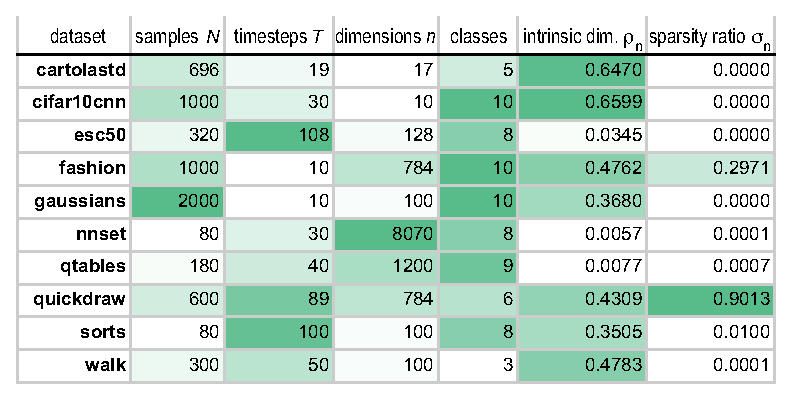
\includegraphics[width=\linewidth]{figures/projection-algorithm/datasets.eps}
% \vspace{-0.15cm}
\end{table}
  
%-------------------------------------------------------------------------
\section{Evaluation results}
\label{sec:results}
%
We used each of the selected 13 projection techniques (Sec.~\ref{sec:eval-methods}) to project the 10 datasets in the benchmark (Sec.~\ref{sec:datasets}). For every (dataset, method) pair, we compute 12 quality metrics (4 related to distance presentation, 4 related to neighborhood preservation, and 4 stability metrics, see Sec.~\ref{sec:metrics}), and analyze the results at different levels of aggregation.
For a direct impression, the animations of each (dataset, method) pair can be found in our online repository \citep{repo-guided}.

%-------------------------------------------------------------------------

% https://docs.google.com/drawings/d/1dUEZz5K3WcL8MpqT95sdXr2dMzeSUX-Vbu6Yg2-1Uv4/edit
%\begin{figure*}[htb!]
%  \centering
%  \includegraphics[width=\linewidth]{figures/projection-algorithm/cifar10grid-with-circles2.pdf}
%  \caption{Trails showing the ``hidden activity''\,\citep{Rauber2017} of a convolutional neural network trained on the \emph{CIFAR10}\,\citep{dataset:cifar10} dataset, computed by all 13 tested dynamic projections. Red circles show clusters of trail endpoints which indicate training convergence. Images without red circles show (suboptimal) projection methods where it is not possible to see this training convergence.}  
%  \label{fig:cifar}
%  \vspace{-0.5cm}
%\end{figure*}


\begin{figure*}[htb!]
  \centering
  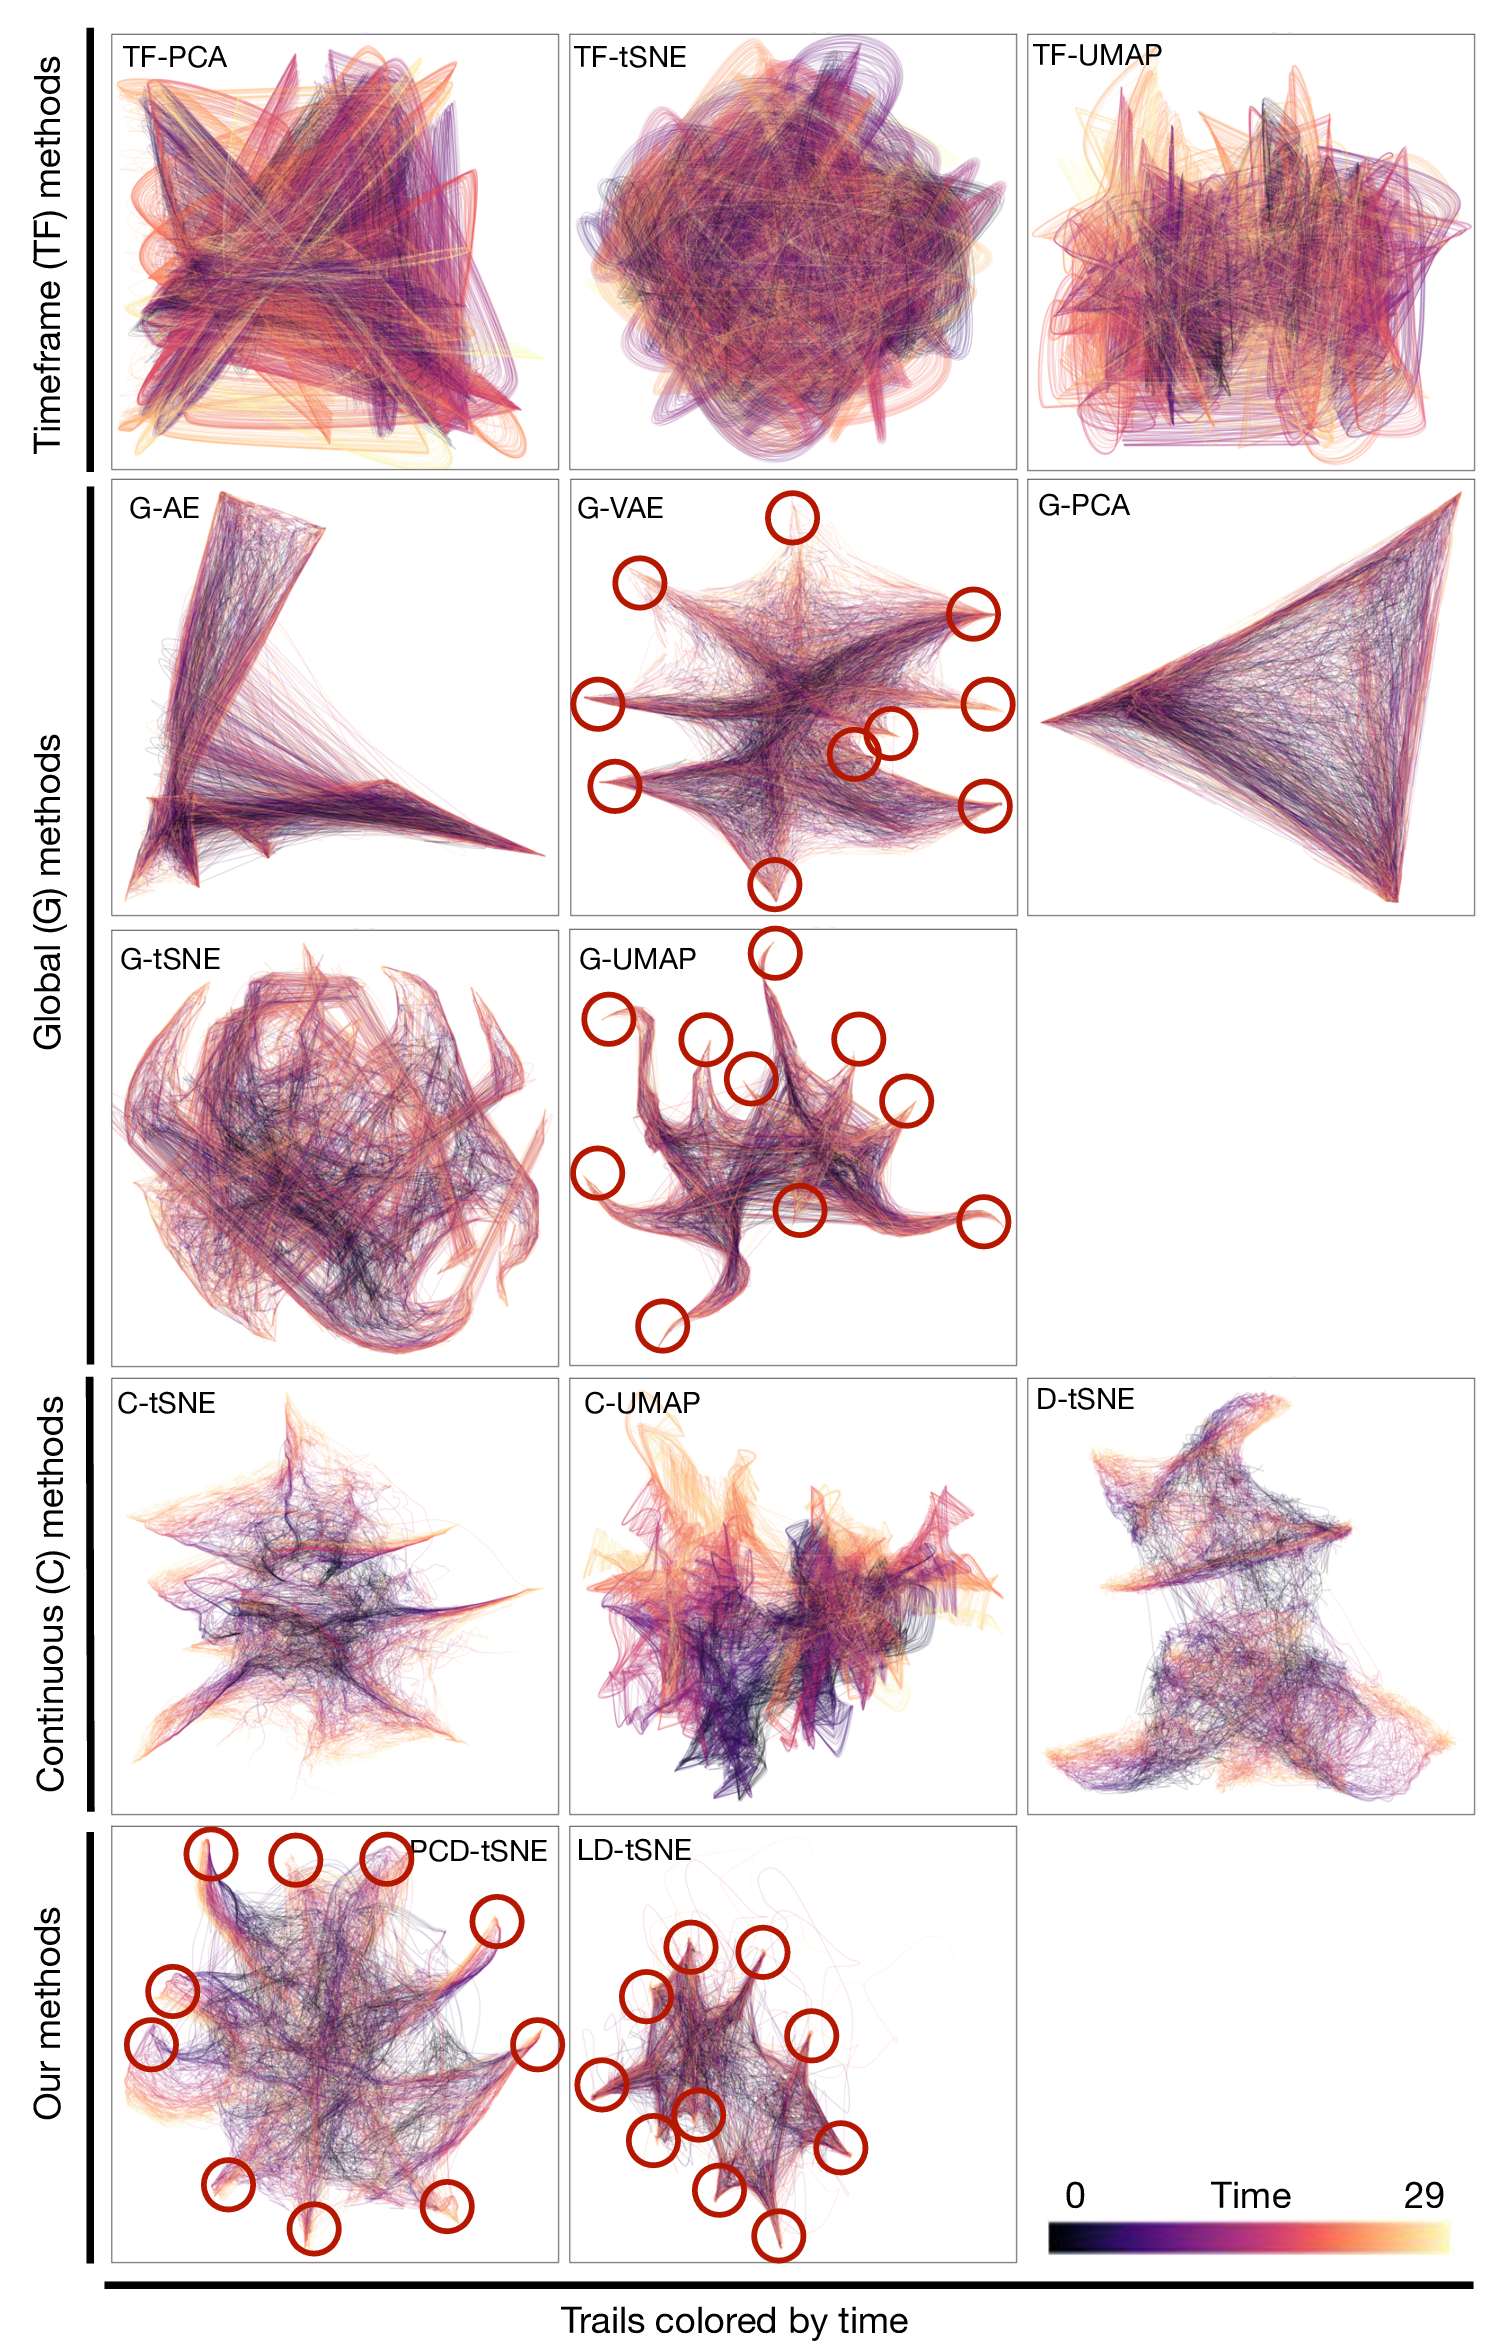
\includegraphics[width=\linewidth]{figures/projection-algorithm/cifar-a.png}
  \caption{Trails showing the ``hidden activity''\,\citep{Rauber2017} of a convolutional neural network trained on the \emph{CIFAR10}\,\citep{dataset:cifar10} dataset, computed by all 13 tested dynamic projections. Red circles show clusters of trail endpoints which indicate training convergence. Images without red circles show (suboptimal) projection methods where it is not possible to see this training convergence.}  
  \label{fig:cifar}
\end{figure*}

\begin{figure*}[htb!]
  \centering
  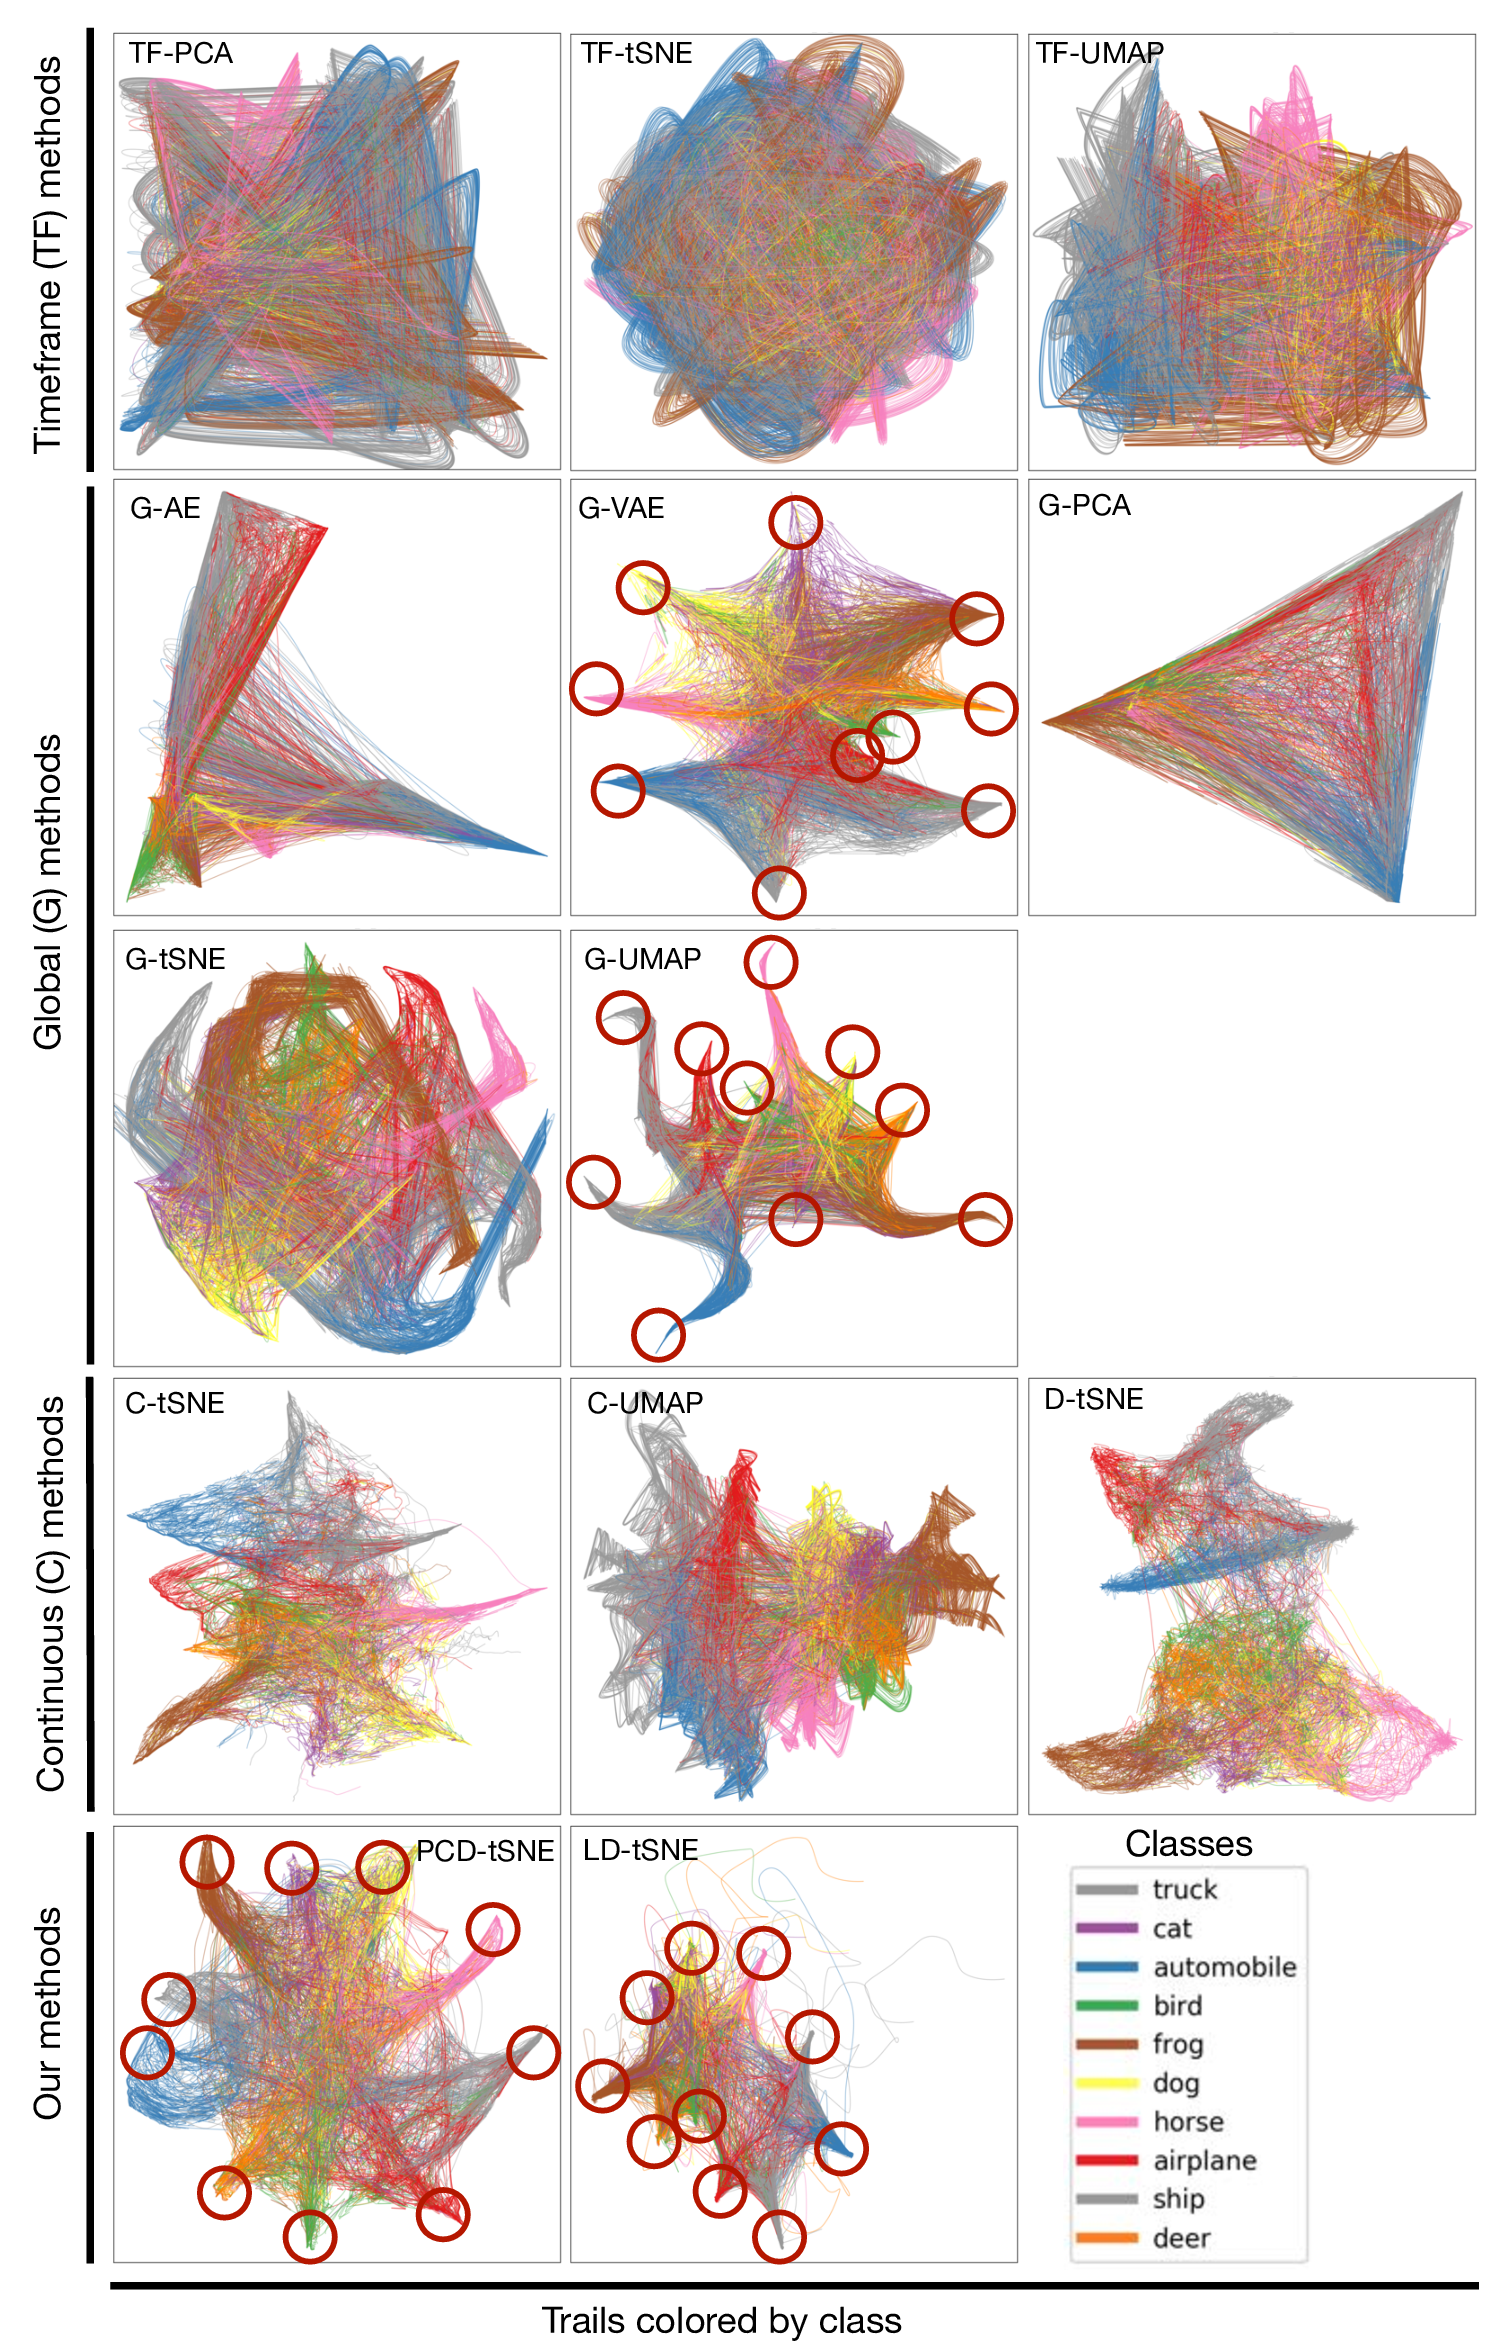
\includegraphics[width=\linewidth]{figures/projection-algorithm/cifar-b.png}
  \caption{Identical trails to \cref{fig:cifar} but colored by data class.}  
  \label{fig:cifar-b}
\end{figure*}


\subsection{Visual comparison of dynamic projections}
\label{sec:visual_comp}
%
We start with a simple, visual comparison of dynamic projection results. Figure~\ref{fig:cifar} shows the trail-sets -- curves linking $P(\mathbf{x}_i^t)$ for all $t$ -- for the \emph{cifar10cnn} dataset, created by the 13 tested dynamic projection methods, organized following the taxonomy in Sec.~\ref{sec:taxonomy}. Points represent the last layer of neural network activations trained to classify the dataset, over 30 training epochs. Given the problem, we \emph{expect} that activations `segregate' into 10 distinct sets, corresponding to the 10 classes of images in the dataset. The trails should start from a roughly common area (middle of the projection), indicating lack of differentiation at training start, and evolve \emph{smoothy}, that is, without major twists and bends, over epochs, to increasingly differentiated clusters, a phenomenon shown earlier in for the (far) easier-to-classify MNIST dataset\,\citep{Rauber2017} by C-tSNE. We see that only a few dynamic projections exhibit this pattern: G-VAE, G-UMAP, and our proposals, PCD-tSNE and LD-tSNE. All other dynamic projections do not show the convergence of trails to (ten) distinct clusters (red circles in the figure). Saliently, all TF variants show far too high dynamics - long trails turning and twisting, suggesting chaotic dynamics, which we know it is not the case from\,\cite{Rauber2017}. Other projections (G-AE, G-PCA, G-tSNE, C-UMAP, D-tSNE) do not show a clear convergence of trails into 10 clusters, which again, we know should be expected. Overall, we argue that PCD-tSNE and LD-tSNE capture the (known) ground-truth of the training dynamics better than most tested counterparts.

\subsection{Overview of quality metrics}
%
Figure \ref{fig:swarm} shows the results for each method separated by metric class. The three swarm plots\,\citep{swarm} in the figure address each of the three metric categories outlined above (distance preservation, neighborhood preservation, temporal stability). Columns in a plot indicate methods. Each point in a column corresponds to the averaged result over the four normalized metrics in the respective class for a (method, dataset) pair. Methods in each plot are ordered by how high they score for a given metric class, with methods to the left scoring higher. Methods are categorically color-coded to ease comparison between the plots.

A method to be considered suitable for dynamic projections must be stable and achieve good distance and neighborhood preservation. Vernier \emph{et al.}'s benchmark \citep{Vernier2020} concluded that, from all their 9 tested methods, G-PCA and Autoencoder-based techniques (G-AE, G-VAE) struck the best balance between these desiderates. We argue that, in this light, our new PCD-tSNE method is even more effective at projecting dynamic data. Indeed, as Fig.~\ref{fig:swarm} (bottom plot) shows, PCD-tSNE's stability is comparable to G-PCA, G-AE, and G-VAE, being the third-most stable of all tested methods. At the same time, PCD-tSNE achieves better results in distance preservation, being the best of all tested methods. Regarding neighborhood preservation (Fig.~\ref{fig:swarm}, middle plot), PCD-tSNE is only surpassed by the TF (timeframe) and C (continuous) methods. This is not surprising since these methods do not have temporal constraints. This implies, as Fig.~\ref{fig:swarm} (bottom plot) confirms, that the TF and C methods score very poorly for stability. 

Additionally, PCD-tSNE overcomes two limitations of AE-based methods and G-PCA: Autoencoders are based on neural networks, which can be challenging to set up, optimize for the architecture, and train; PCA based methods are sensitive to outliers and do not explicitly try to preserve local features.

Concerning LD-tSNE, we see that this method did not achieve metric results as good as other state-of-the-art methods. Yet, it scores in the top half of all methods for all three considered metric classes. Also, its strength lies in its customizability (see next Sec. \ref{sec:landmark-placement}): If we want the projection to adhere to a certain shape, or we have some prior knowledge over the high-dimensional space and we want areas of the projections to carry a certain data-related semantic, we can easily place landmarks to drive the projection to that behavior. This extends the same flexibility, known earlier for static projections (see \emph{e.g.}\,\citep{Joia2011,Pekalska1999}), to dynamic projections.

\begin{figure}[htb!]\centering
 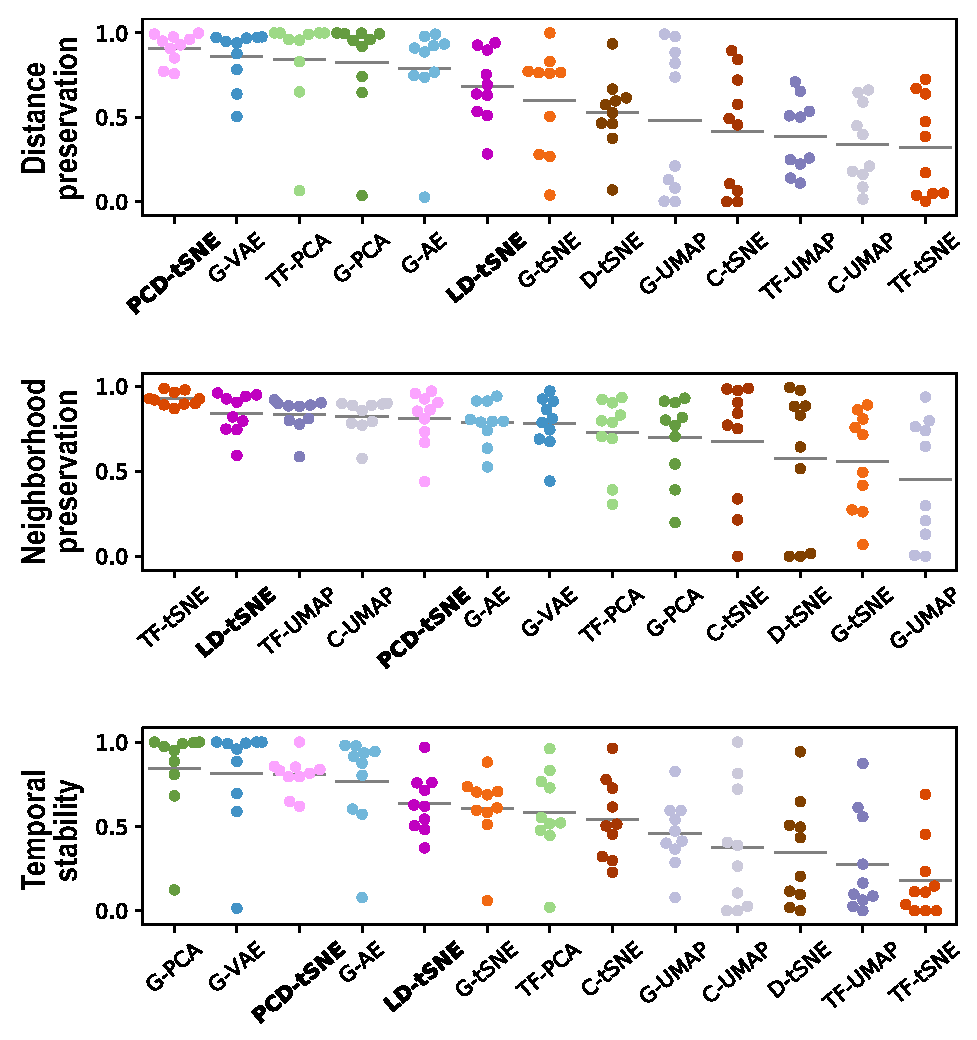
\includegraphics[width=0.92\linewidth]{figures/projection-algorithm/swarm.eps}
 \vspace{-0.25cm}
 \caption{
  Swarm plot ordering methods from best to worse for each metric class.
  Each point corresponds to the average metric result over the 4 metrics in a given class normalized to $[0,1]$ for each (method, dataset) pair.
  Horizontal lines show average metric values over all datasets for each (method, metric class) pair.
 }
 \vspace{-0.25cm}
 \label{fig:swarm}
\end{figure}

%-------------------------------------------------------------------------
\subsection{Stability and spatial quality trade-off}
\label{sec:starplot}
%
While the swarm plots in Fig.~\ref{fig:swarm} help us see which methods score best for a given metric class, they do not let us easily compare methods from the perspective of \emph{multiple} metrics. To achieve this, we use two star plots (Fig.~\ref{fig:star}), as follows. Each image is a scatterplot having temporal stability as the $x$ axis and distance and neighborhood preservation, respectively, as the $y$ axis. Each colored point shows the average metric values for a given technique over all datasets. Spokes emerging from a point show the average metric values for each of the 10 datasets run by the respective technique. For more insight into the behavior of the methods, we highlighted the spokes for the two best methods in each plot, \emph{i.e.} the points placed closest to the top-right corner of the plot. 

Figure~\ref{fig:star}a shows that PCD-tSNE and G-VAE are the best methods for distance preservation \emph{and} stability, closely followed by G-PCA. Yet, the spokes of PCD-tSNE (pink) are shorter than those of G-VAE (blue). That is, PCD-tSNE achieves a consistently higher distance preservation and stability over all 10 tested datasets than G-VAE, which has a higher variability. Similarly, Figure~\ref{fig:star}b shows that PCD-tSNE scores highest in terms of neighborhood preservation \emph{and} stability, closely followed by G-VAE and G-AE. Again, the spokes of PCD-tSNE are shorter than those of G-VAE, telling that PCD-tSNE achieves its high scores more consistently than G-VAE. We see that G-VAE performs worst for the \emph{walk}, \emph{nnset}, and \emph{fashion} datasets, from both the perspective of distance preservation and neighborhood preservation (longest blue spokes in Figs.~\ref{fig:star}a,b for G-VAE, indicated by a cross, triangle, and check icons); for these datasets, PCD-tSNE performs quite well (short pink spokes). Also, there seems to be an inverse correlation between neighborhood and distance preservation for TF-tSNE, TF-UMAP, and G-UMAP, indicating that these methods are very good at neighborhood, but not distance, preservation. Separately, we see that our two methods, PCD-tSNE and LD-tSNE, are the best methods, stability-wise, from the t-SNE class, and perform far better, on all three metrics, than D-tSNE. In other words, if one wants to leverage t-SNE's ability for dynamic datasets, our methods are the best from the considered variants. Finally, we see that temporal stability and distance preservation appear to be well correlated over all tested methods (points in Fig.~\ref{fig:star}a close to the diagonal), which is to our knowledge a new finding in the projection literature. In contrast, no similar correlation appears between stability and neighborhood preservation (Fig.~\ref{fig:star}b).


% https://docs.google.com/drawings/d/1ILKutH7vsdBAuz4Gd6PnaYQzuvehAU3Jy8q83Z6PCEA/edit
\begin{figure}[htb!]\centering
 \includegraphics[width=.73\linewidth]{figures/projection-algorithm/labbeled-starplot.pdf}
 \vspace{-0.2cm}
 \caption{Star plots compare dynamic projection methods from the perspective of stability \emph{vs} distance (a) and stability \emph{vs} neighborhood (b) preservation. A point shows the average values of these metrics for a given technique over all datasets. Spokes show the average metric values for each dataset for a given technique. Spokes of PCD-tSNE and VAE, the two techniques that score best, are in bold. Methods with big spoke fans show high variation on quality metrics. Short spokes show consistent results of a method over all 10 datasets.}
 \vspace{-0.5cm}
 \label{fig:star}
\end{figure}

%-------------------------------------------------------------------------
\subsection{Global \emph{vs} local influence control}
\label{sec:lambda}

As outlined in Sec. \ref{sec:pcd-tsne}, the PCD-tSNE method has a parameter $\lambda$ that modulates the amount of global influence applied to the points being projected. 
When projecting a sample $\mathbf{x}_i \in \mathbf{D}$, this global influence refers to minimizing the distance of $P(\mathbf{x}_i)$ to the position given by the transformation matrix $W$ composed of the top-$q$ eigenvectors of $\mathbf{D}$. 
Another way to interpret this global influence is to think of $\mathbf{x}_{i} W$ as the position that G-PCA would generate; and to think about $\lambda$ as how much we want PCD-tSNE to approximate G-PCA.

If we use high $\lambda$ values (close to 1), PCD-tSNE gets very close to G-PCA, a method that has shown to be very stable, produce good distance preservation, but has low neighborhood preservation (Fig.~\ref{fig:swarm}). Conversely, 
with low $\lambda$ values (close to 0), no global influences act upon PCD-tSNE, which turns into C-tSNE, a method that has high neighborhood preservation, but low stability and distance preservation (Fig.~\ref{fig:swarm}). 
Figure~\ref{fig:lambda} supports and refines this insight. For each dataset (rows), we compute the mean distance preservation (MDP), mean neighborhood preservation (MNP), and mean temporal stability (MTS) over the respective metrics in each class (see Sec.~\ref{sec:metrics}). For each table row, we normalize values between 0 and 1, to better see the spread of values of the respective metric for each dataset.
The leftmost column shows the metric results of G-PCA; the rightmost one shows the results of C-tSNE. The six middle columns
show the results of PCD-tSNE with $\lambda$ in $\{10^{-2}, 10^{-3}, 10^{-4}, 10^{-5}, 10^{-6}, 10^{-7}\}$. Cells are colored using an ordinal colormap (dark green=low, bright yellow=high metric values) on the normalized values. The color gradients show that PCD-tSNE indeed yields metric values that are very similar, for high, respectively low, $\lambda$ to those of G-PCA, respectively C-tSNE. Also, we see that PCD-tSNE can integrate characteristics of both C-tSNE and G-PCA and achieves the best balance between all quality metrics, as shown by the overall brightest columns in the middle of the table. Interestingly, PCD-tSNE is also often able to achieve the best result for certain quality metrics (maximum averages, marked bold in Fig.~\ref{fig:lambda}). This shows that PCD-tSNE doesn't simply \emph{interpolate} projections (like, for example, in\,\cite{kruiger_mdpi}), but uses the characteristics of both C-tSNE and G-PCA to create a better projection. In Fig.~\ref{fig:lambda}, note that different rows show different trends, which is expected since we consider different datasets and metrics. 

Finally, Figure~\ref{fig:lambda} shows that G-PCA and C-tSNE are not always optimal -- the best projection lies sometimes in between, which is what PCD-tSNE obtains. Separately, it shows that optimal parameters depend on the dataset. The considered MDP, MNP, and MTS quality metrics could be used for automatic finding of such optimal parameters -- or good preset values for all datasets -- by grid search, following the approach in\,\cite{Espadoto19} for static projections.

% https://docs.google.com/drawings/d/18Y6EjHYnk1McBokhSRCSHwiHzoDtwdT-Ddccpk9r-og/edit
\begin{figure}[htb!]\centering
 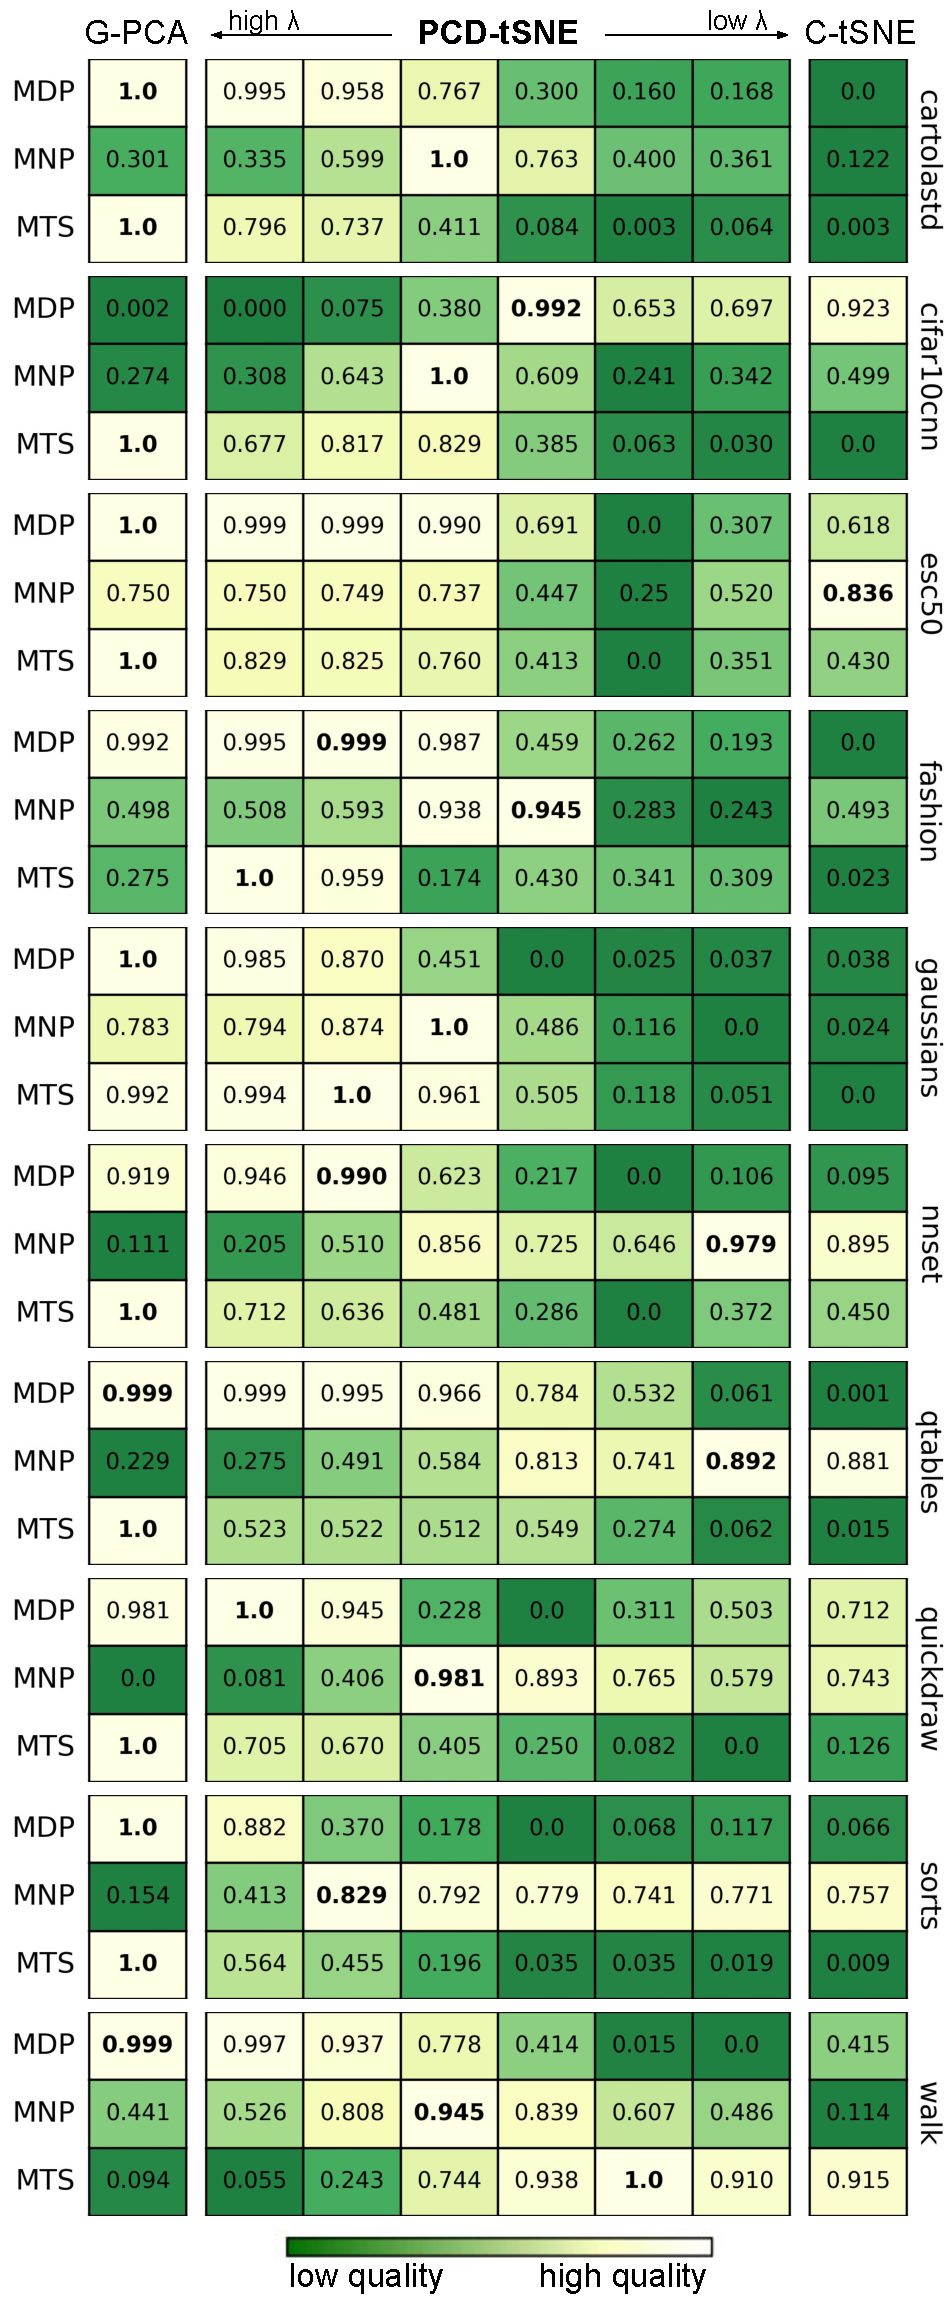
\includegraphics[width=.7\linewidth]{figures/projection-algorithm/lambda-influence-on-metrics.pdf}
 \caption{
Mean distance preservation (MDP), mean neighborhood preservation (MNP), and mean temporal stability (MTS) per dataset, as in Figs.~\ref{fig:swarm} and~\ref{fig:star}, but normalized over the 8 runs in each subplot.
  The leftmost column is for G-PCA. The next 6 columns are for PCD-tSNE with $\lambda \in \{10^{-2}, 10^{-3}, 10^{-4}, 10^{-5}, 10^{-6}, 10^{-7}\}$. The rightmost column is for C-tSNE.
  By changing $\lambda$, PCD-tSNE generates a smooth gradient, simulating G-PCA and C-tSNE at the extremes and producing hybrids in-between (Sec.~\ref{sec:pcd-tsne}). The best balance between all metric classes is often found in this compromise.}
  \vspace{-0.5cm}
 \label{fig:lambda}
\end{figure}

%-------------------------------------------------------------------------


\subsection{Using landmarks to steer dynamic projections} 
\label{sec:landmark-placement}
%
The key trait of LD-tSNE is that it allows steering a \emph{dynamic} projection by changing the landmark point positions $\mathbf{l}^q$. If we monitor a high-dimensional process and we know what final and failed states look like, we can place landmarks indicating these states. As the process evolves, we will have a clear picture of which samples failed or succeeded; which samples are on the ``right track''; and how similar samples are in in-between states among themselves and to these known states. Guiding landmarks are also valuable if we want a system that is consistent over slightly different datasets. 

Landmark-based methods present many challenges in practice: How to choose a small set of points in $\mathbb{R}^n$ that is representative of $\mathbf{D}$? How many points do we need, and how do we select these representatives? \cite{DeSilva2005} propose regression models for picking the best landmarks, while \cite{Pezzotti2016} use a hierarchical approach. Another option is to synthesize landmarks using models that approximate the manifold (e.g. Autoencoders). For simplicity, we select our landmarks by random sampling $\mathbf{D}$, as in earlier work considering static projections, \emph{e.g.}\,\citep{Joia2011,Pekalska1999}.

Figure~\ref{fig:landmark-placement} shows how landmark placement can steer a dynamic projection. We use the \emph{gaussians} dataset, as we know its dynamics, so we can assess how well landmark steering works on the resulting projections. Points are colored per cluster; landmarks are drawn white. Figure~\ref{fig:landmark-placement}a shows several timesteps of LD-tSNE with landmarks placed by G-PCA. We see how clusters `implode' over time. While clusters stay roughly in the same place over time in the projection (a good indication of stability), their \emph{spatial} organization is not ideal for monitoring the phenomenon. Figure~\ref{fig:landmark-placement}b shows LD-tSNE for the same dataset, with the same landmarks $\mathbf{l}^n$ selected from $\mathbf{D}$, but with the 2D landmarks $\mathbf{l}^q$ placed manually into 10 horizontally-aligned, similar-size, clusters. The images show the same `implosion' effect over time as in Fig.~\ref{fig:landmark-placement}a. We argue that the \emph{dynamics} of the data is now much easier to see due to the separation of clusters given by our 2D landmarks' placement. The point made is that the freedom of landmark placement of LD-tSNE allows one to separate the issues of spatial disentanglement of samples in the projection (done by the landmark placement) from monitoring the dynamics of the data (taken care of by LD-tSNE). The Appendix (supplementary material) shows additional information on this and related experiments.

%Imagine we are tracking groups of patients in trial groups, and we want the $qD$-space to be coherent over the different groups
%(something similar could be done by locking the Principal Components in PCD-tSNE or G-PCA, but we wouldn't have control over the position of certain states). \alex{This is highly speculative, we don't show anything like this, so remove.}

%\red{talk about how difficult it is to choose nD representatives (how many landmarks do we want, sampling vs generating), and that different ways of projecting or manually placing those representatives into 2D will generate very different projections}

%\red{
%  Here I'm trying to show that by changing the position of the landmarks, we can steer the projection to a certain desired shape while still preserving the overall dynamics of the dataset. \\
%  This can be useful in tasks that envolve event monitoring, for example, or if you have area in nD that you know has some semantic attached to it. 
%}

% https://docs.google.com/drawings/d/1TKqYarp4TPveX8jyZx8E_A6-T2bSKxPmIFcOUgbj3ro/edit
\begin{figure}[h]\centering
 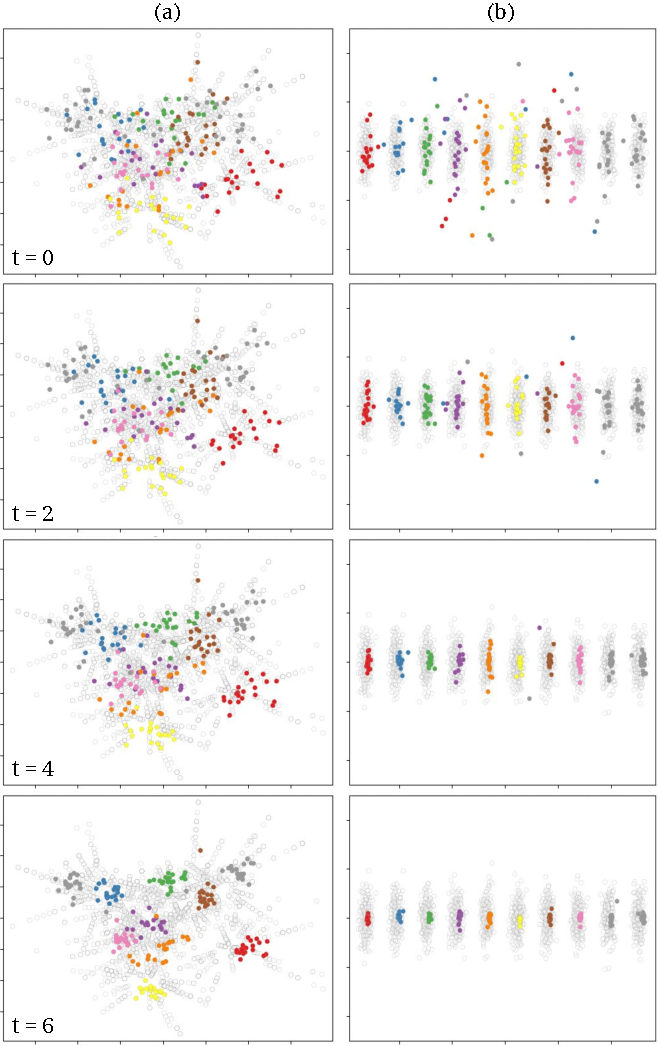
\includegraphics[width=0.95\linewidth]{figures/projection-algorithm/landmark-placement.pdf}
 \caption{Projection of the \emph{gaussians} dataset with landmarks (gray points) placed (a) by G-PCA and (b) manually according to cluster label. Points are colored by cluster label. The implosion dynamics known to be present in the data is visible in both cases. Yet, the manual landmark placement creates a less cluttered view.}
 \label{fig:landmark-placement}
 \vspace{-0.5cm}
\end{figure}


%-------------------------------------------------------------------------

\section{Conclusion}
\label{sec:conclusion-5}
%
We have presented two projection methods that leverage the good neighborhood-preservation ability of t-SNE for dynamic (time-dependent) data. For this, we use guidance in the form of landmarks (for our first method, LD-tSNE), respectively attractors to principal vectors (for our second method, PCD-tSNE). We compared our methods against 11 dynamic projection techniques on 10 datasets using 8 spatial quality and 4 stability metrics. The comparison showed that PCD-tSNE scores better than all compared methods on the combined spatial quality and stability criteria. LD-tSNE obtained second-best scores on neighborhood preservation, allowing flexible placement of landmarks to drive the shape of the resulting dynamic projection. While our work -- for sure -- does not solve the problem of dynamic projection of high-dimensional data, we argue that our methods bring added value to users interested in this goal.

We next aim to extend our methods to handle streaming data. Adapting our work to use deep learning, similar to\,\cite{MateusEspadoto}, would lead to high-quality and computationally scalable dynamic projections. Additional validation of our methods on more datasets, and with concrete use-cases and user tasks, is also important. Finally, developing new metrics to measure the quality of dynamic projections for specific tasks, thereby extending the insights in\,\cite{Nonato2019} for the dynamic case, is a long-term goal we aim to pursue.

